% !TeX root = RJwrapper.tex
\title{Generalized Mosaic Plots in the ggplot2 Framework}
\author{by Haley Jeppson and Heike Hofmann}

\maketitle

\abstract{%
Graphical methods for categorical variables are not well developed when compared with visualizations for numeric data. One method available for multidimensional categorical data visualizations is mosaic plots. Mosaic plots are an easy and powerful option for identifying relationships between multiple categorical variables. Although various packages have implemented mosaic plots, no implementation within the grammar of graphics supports mosaic plots. We present a new implementation of mosaic plots in R, \pkg{ggmosaic}, that implements a custom \pkg{ggplot2} geom designed for generalized mosaic plots. Equipped with the functionality and flexibility of \pkg{ggplot2}, \pkg{ggmosaic} introduces new features not previously available for mosaic plots, including a novel method of incorporating a rendering of the underlying density via jittering. This paper provides an overview of the implementation and examples that highlight the versatility and ease of use of \pkg{ggmosaic} while demonstrating the practicality of mosaic plots.
}

\hypertarget{introduction}{%
\section{Introduction}\label{introduction}}

Graphical methods for categorical variables are not as thoroughly developed when compared with what is available for numeric variables. Categorical variables in scientific publications often appear in the form of bar charts (first published in the Commercial and Political Atlas by William Playfair in 1789, re-edited by Playfair, Wainer, and Spence (2005)) and spine plots (Hummel 1996).

Beyond those visualizations, categorical variables with a low number of levels are often incorporated in visualizations in the form of aesthetics such as color and shape. However, these indirect methods of visualizing categorical information are better suited as supplemental information and not as the primary source of information due to the associated loss of accuracy in retrieving the corresponding information (Cleveland and McGill 1984).

Mosaic plots provide a direct method of visualizing multidimensional categorical data; they are similar to a stacked bar chart but include the marginal distribution in addition to the conditional distribution, can be extended beyond two variables, and provide additional flexibility. Modern mosaic plots are usually attributed to Hartigan and Kleiner (Hartigan and Kleiner 1981, 1984; Kleiner and Hartigan 1981), but historical versions of mosaic plots can be found as far back as the late 1800s. The first mosaic plot is often attributed to Georg von Mayr (Friendly 2002); however, the mosaic plots in the Statistical Atlas of the 1870 Decennial Census (United States Census office. 9th census, 1870 and Walker 1874) pre-dates Mayr's by a few years. Mosaic plots may also be identified as Marimekko charts (mainly in the InfoVis world) or Eikosograms (Oldford et al. 2018).

In R, mosaic plots have been implemented in a variety of packages. Base R is equipped with the function \texttt{mosaicplot()} from the graphics package based on code by Emerson (1998) adapted by Kurt Hornik. The base R generic function \texttt{plot()} contains a method for \texttt{table} objects and produces a mosaic plot from a contingency table using the \texttt{mosaicplot()} function. Similarly, the \CRANpkg{yardstick} package (Kuhn, Vaughan, and Hvitfeldt 2022) provides a method for the \CRANpkg{ggplot2} (Wickham et al. 2020) function \texttt{autoplot()} to visualize confusion matrices, with one of the options being a mosaic plot.

The \CRANpkg{vcd} package (Meyer, Zeileis, and Hornik 2020), influenced by Michael Friendly's ``Visualizing Categorical Data,'' provides the functions \texttt{mosaic()} and \texttt{strucplot()} which allow for expanded versions of the original mosaic plot (Hartigan and Kleiner 1981). The \pkg{eikosogram} package (Oldford et al. 2018) is another R package capable of producing mosaic plots. The function \texttt{tileplot()} in the \CRANpkg{latticeExtra} package (Sarkar and Andrews 2016) provides functionality to create mosaic plots in the \CRANpkg{lattice} framework (Sarkar 2020).

The \CRANpkg{productplots} package (Wickham and Hofmann 2016) provides a wrapper of \pkg{ggplot2} functionality but does not provide universal access to all aspects of the \pkg{ggplot2} framework like a geom does. The left plot in Figure \ref{fig:prodplot} is an example of a mosaic plot created with the \pkg{productplots} package. While the default plot can be annotated with additional aesthetics, labels, themes, and color schemes, we can not add layers to this plot, and faceting is unavailable. A preview of the relevant code follows the next paragraph.

We present a new implementation of mosaic plots in R, \CRANpkg{ggmosaic}, that implements a \pkg{ggplot2} geom for mosaic plots. While several other packages are available for constructing mosaic plots, \pkg{ggmosaic} allows users to fully leverage the widely used \pkg{ggplot2} framework resulting in a flexible package for generalized mosaic plots. More noteworthy, \pkg{ggmosaic} introduces several new features not previously available for mosaic plots, including a novel method of incorporating a rendering of the underlying density via jittering. \pkg{ggmosaic} includes a Shiny app to preview plots interactively and allow for model exploration. Many of the features we describe are possible because \pkg{ggmosaic} is implemented within the architecture defined by \pkg{ggplot2}. A preview of the syntax used in \pkg{ggmosaic} is shown below compared to that of the \pkg{productplots} package. The resulting plot is the right plot of Figure \ref{fig:prodplot}.

\begin{verbatim}
# productplots
productplots::prodplot(flights, ~do_you_recline + rude_to_recline, mosaic()) + 
  aes(fill = do_you_recline)

## ggmosaic
ggplot(data = flights) +
   geom_mosaic(aes(x = product(do_you_recline, rude_to_recline),
                   fill = do_you_recline))
\end{verbatim}

\begin{figure}

{\centering 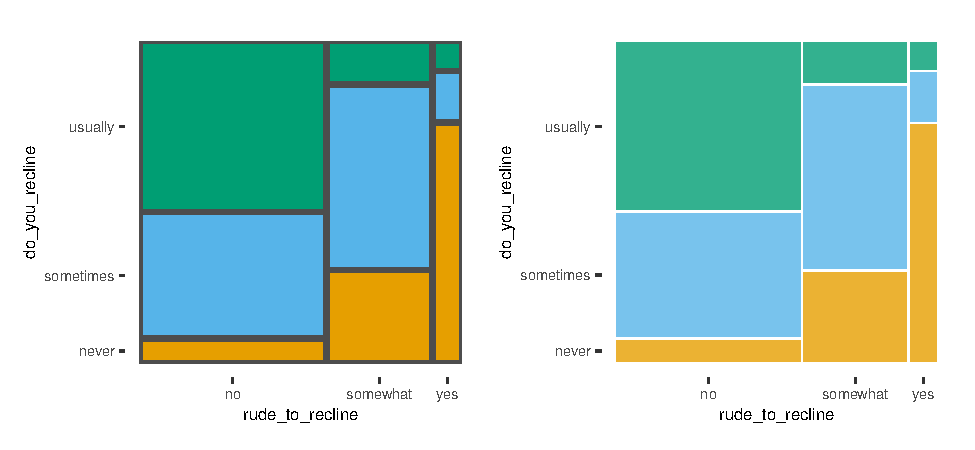
\includegraphics[width=1\linewidth]{RJ-2023-013_files/figure-latex/prodplot-1} 

}

\caption{Example mosaic plots made with the productplots package (left) and the ggmosaic package (right). While the differences are subtle in this basic example, the differences between the two packages become more apparent as the customization of the mosaic plot increases.}\label{fig:prodplot}
\end{figure}

In this paper, we motivate the \pkg{ggmosaic} implementation and introduce it with examples demonstrating the versatility and ease of use of \pkg{ggmosaic}. Next, we describe new features available in the latest release of \pkg{ggmosaic}, version 0.3.3, and discuss how these features can enhance the data visualizations made with \pkg{ggmosaic}. Finally, we conclude with a preview of a \CRANpkg{shiny} application (Chang et al. 2021) designed for an exploratory model framework of logistic regression and loglinear models. The Shiny application is included in the development version of \pkg{ggmosaic} available from \url{https://github.com/hjeppson/ggmosaic}.

\hypertarget{a-implementation-of-mosaic-plots}{%
\section{\texorpdfstring{\pkg{ggmosaic}: A \pkg{ggplot2} implementation of mosaic plots}{: A  implementation of mosaic plots}}\label{a-implementation-of-mosaic-plots}}

\pkg{ggplot2} implements an adaptation of the grammar of graphics (Wilkinson 1999), a layered grammar (Wickham 2010). Because of its flexibility and ease of use, \pkg{ggplot2} has become one of the most popular plotting packages available in the R ecosystem. Version 2.0.0 of \pkg{ggplot2} introduced a method for other R packages to implement custom geometries, or ``geoms'', allowing for an expansion of the utility of \pkg{ggplot2}. In turn, the increasingly popular package has continued to appeal to a more extensive user base.

In creating a \pkg{ggplot2} geom for mosaic plots, we seek to appeal to this user base and leverage the robust framework of the grammar of graphics. Having mosaic plots in the \pkg{ggplot2} framework makes creating mosaic plots more accessible as it is more straightforward for the novice user to create mosaic plots for data exploration purposes. For many users, having mosaic plots function as a true \pkg{ggplot2} geom reduces the amount of syntax required, eliminates the need for prior calculations, and provides complete access to additional benefits of \pkg{ggplot2}, allowing for highly customized generalized mosaic plots.

With the R package \pkg{ggmosaic}, a custom \pkg{ggplot2} geom designed for generalized mosaic plots is implemented. \pkg{ggmosaic} makes mosaic plots compatible with \pkg{ggplot2} and creates a flexible method to generate a wide variety of categorical data visualizations. The remainder of the paper presents a thorough description of the \pkg{ggmosaic} package featuring examples that go beyond how to use \pkg{ggmosaic} and demonstrate how to make more informed decisions about how to use mosaic plots to answer various questions.

We begin with an introduction to the package with examples of the flexible framework that \pkg{ggmosaic} offers. The following three sections illustrate how to use \pkg{ggmosaic}. First, we address the data structures required for constructing mosaic plots and which structures are compatible with \pkg{ggmosaic}. Next, we demonstrate how \pkg{ggmosaic} fits mosaic plots into the \pkg{ggplot2} framework and how to define the aesthetic mappings to construct the desired plot from the variables in the data. Lastly, we provide examples of mosaic plots customized with parameters unique to \pkg{ggmosaic}.

The remaining half of the paper presents the new features included in version 0.3.3 of \pkg{ggmosaic}. Frist, we introduce \texttt{geom\_mosaic\_text()}, designed to place text, or labels, in the center of each tile, followed by \texttt{geom\_mosaic\_jitter()}, a geom for jittered points designed to be superimposed on the mosaic plot and with multiple proposed applications. Next, we present \texttt{theme\_mosaic()}, a theme for mosaic plots to remove items from the background of the plot. We conclude with an overview of an interactive Shiny app for exploratory data analysis (EDA) of high-dimensional categorical data using mosaic plots.

Many of the features we describe are possible because \pkg{ggmosaic} is implemented within the \pkg{ggplot2} framework. While other packages are available for constructing mosaic plots, \pkg{ggmosaic} allows users to leverage the widely used \pkg{ggplot2} infrastructure to create highly customized generalized mosaic plots. Most notably, \pkg{ggmosaic} introduces several new features not previously available for mosaic plots. In total, \pkg{ggmosaic} offers users a way to make mosaic plots with \pkg{ggplot2} to visualize and explore categorical data more effectively.

\hypertarget{the-package}{%
\section{\texorpdfstring{The \pkg{ggmosaic} package}{The  package}}\label{the-package}}

The R package \pkg{ggmosaic} implements a custom \pkg{ggplot2} geom, \texttt{geom\_mosaic()}, designed to offer a flexible framework for visualizing categorical data. The geom for mosaic plots was created using the \pkg{productplots} package and \pkg{ggplot2}'s custom object-oriented system and extension mechanism, ggproto. A stable version of \pkg{ggmosaic} is available on CRAN, and a development version is available at \url{https://github.com/hjeppson/ggmosaic}. This section provides a brief description of the package, the methods used in its implementation, and an example that showcases the flexibility that \pkg{ggmosaic} offers.

Designed to create visualizations of categorical data, \texttt{geom\_mosaic()} has the capability to produce bar charts, stacked bar charts, mosaic plots, and double-decker plots and therefore offers a wide range of potential plots. Figures \ref{fig:variety1}, \ref{fig:variety2}, and \ref{fig:variety3} highlight the package's versatility. The code for these examples is provided below and can be summarized as consisting of the following components. First, the mosaic plot is created by adding a mosaic geom. The \texttt{x} aesthetic takes one or more variables wrapped in the \texttt{product()} function, and the \texttt{fill} aesthetic determines the fill color of the rectangles. An optional \texttt{divider} parameter determines the partitioning strategy for the rectangles. The code will be explained in greater detail in the subsequent sections.

\begin{verbatim}
# one-dimensional examples:
# spine plot
ggplot(data = flights) + 
  geom_mosaic(aes(x = product(do_you_recline), 
                  fill = do_you_recline))

# bar chart
ggplot(data = flights) + 
  geom_mosaic(aes(x = product(do_you_recline),
                  fill = do_you_recline), 
              divider = "hbar") 
\end{verbatim}

\begin{figure}[!h]

{\centering 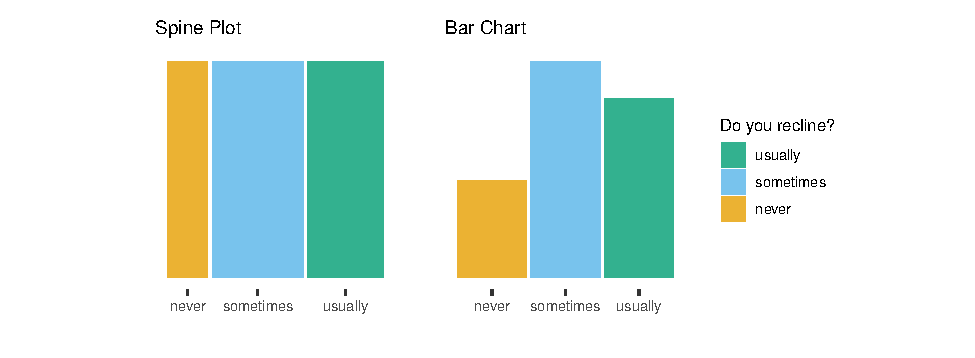
\includegraphics[width=1\linewidth]{RJ-2023-013_files/figure-latex/variety1-1} 

}

\caption{Both plots represent the distribution of \code{do\_you\_recline} and allow the same comparisons, though the spine plot does so with proportions and the bar chart with frequencies. The relative group sizes are more difficult to compare in the spine plot, but the \code{"sometimes"} group is still discernable as the largest and the \code{"never"} group as the smallest. The bar chart provides an easier comparisons of the relative group sizes.}\label{fig:variety1}
\end{figure}

\begin{verbatim}
# two-dimensional examples:
# mosaic plot (2 variables)
ggplot(data = flights) +
  geom_mosaic(aes(x = product(do_you_recline, rude_to_recline), 
                  fill = do_you_recline))

# stacked bar chart
ggplot(data = flights) + 
  geom_mosaic(aes(x = product(do_you_recline, rude_to_recline), 
                  fill = do_you_recline),
              divider = c("vspine", "hbar"))
\end{verbatim}

\begin{figure}[!h]

{\centering 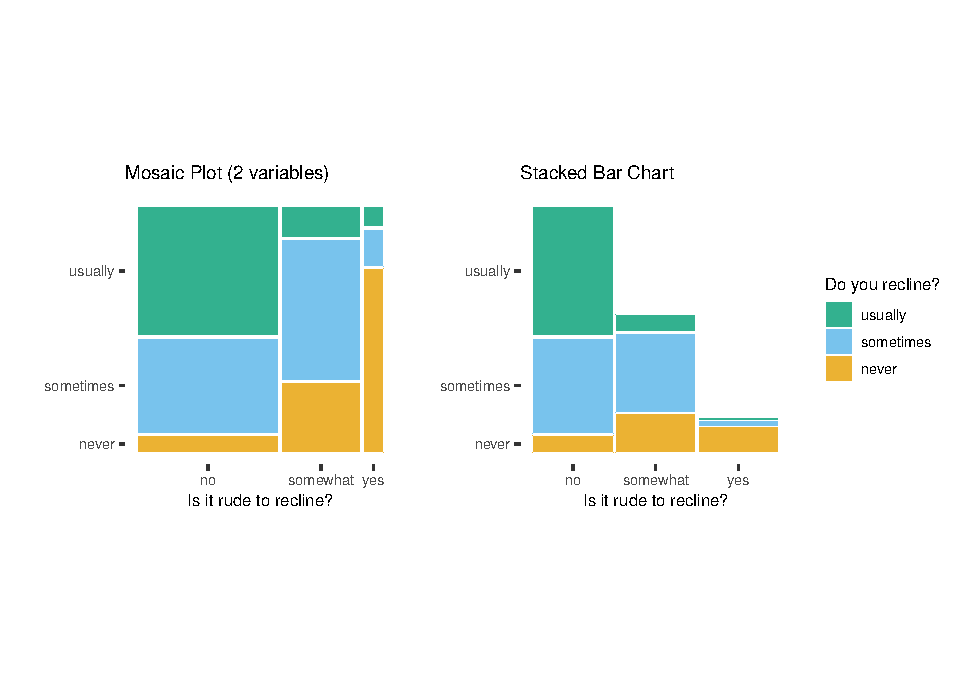
\includegraphics[width=1\linewidth]{RJ-2023-013_files/figure-latex/variety2-1} 

}

\caption{The conditional distribution of \code{do\_you\_recline} given \code{rude\_to\_recline} is represented by the heights of the bars in both the mosaic plot (left) and the stacked bar chart (right). The mosaic plot displays the joint and marginal distribution of \code{rude\_to\_recline} with the area and width of the tile, respectively. The stacked bar chart reveals a nearly equal number of never reclining responses across the categories of \code{rude\_to\_recline}. The conditional probabilities of \code{"never"} given \code{"somewhat"} and \code{"never"} given \code{"yes"} have a more significant impact in the mosaic plot, from which we understand that there is a positive correlation between a respondent considering reclining to be rude and electing never to recline their seat. There are, however, respondents that do not consider reclining to be rude and yet never recline, and perhaps more egregious, there are those that do regard reclining as rude and yet usually recline their seats, a group that is important in the mosaic plot but challenging to see in the stacked bar chart.}\label{fig:variety2}
\end{figure}

\begin{verbatim}
# three-dimensional examples:
# mosaic plot (3 variables)
ggplot(data = flights) +
  geom_mosaic(aes(x = product(eliminate_reclining, do_you_recline,
                              rude_to_recline),
                  fill = do_you_recline, 
                  alpha = eliminate_reclining))

# double-decker plot
ggplot(data = flights) +
  geom_mosaic(aes(x = product(do_you_recline, eliminate_reclining,
                              rude_to_recline), 
                  fill = do_you_recline, 
                  alpha = eliminate_reclining),
              divider = ddecker())
\end{verbatim}

\begin{figure}[!h]

{\centering 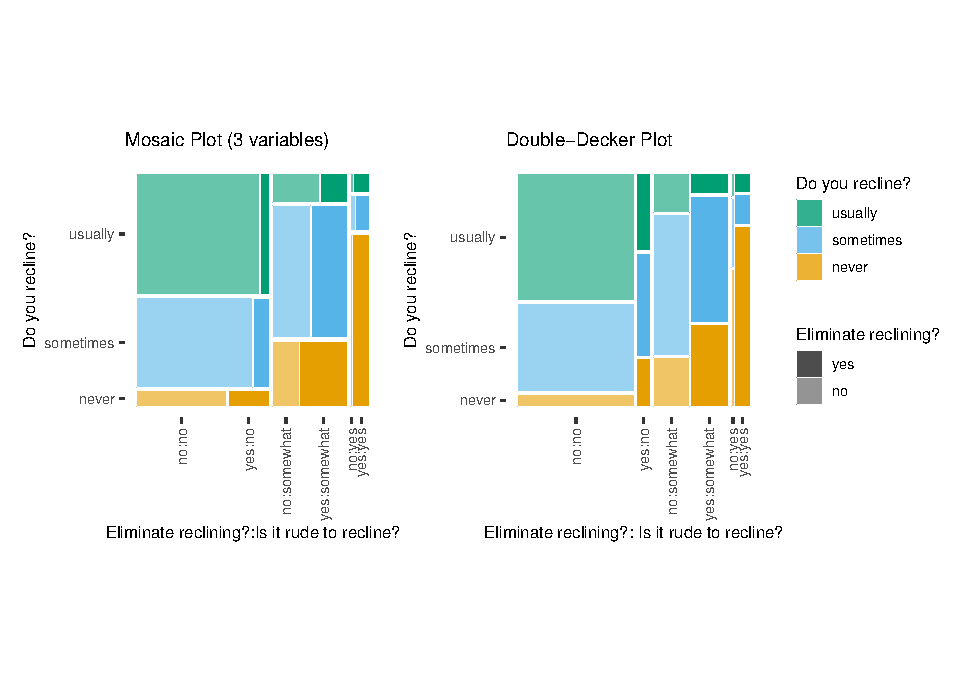
\includegraphics[width=1\linewidth]{RJ-2023-013_files/figure-latex/variety3-1} 

}

\caption{The mosaic plot (left) and double-decker plot (right) include the three variables (\code{do\_you\_recline}, \code{rude\_to\_recline}, \code{eliminate\_reclining}), though the direction of the splits varies between the two plots. Both plots display a connection between a passenger's opinions of reclining and their tendency to recline. Those that consider reclining to be rude are less likely to recline and more likely to wish for reclining to be eliminated. The mosaic plot reveals an increasing desire to eliminate reclining when the respondents believe reclining to be rude across all categories of \code{do\_you\_recline}. There appears to be a slight positive correlation between reclining and not electing to eliminate reclining across all levels of \code{rude\_to\_recline}. The double-decker plot (a mosaic plot with a specific structure) best highlights the conditional distribution of \code{do\_you\_recline} and allows for easier comparisons across the categories of the other two variables. For example, the relationship between \code{do\_you\_recline} and \code{eliminate\_reclining} seems consistent across categories of \code{rude\_to\_recline}, a conclusion that is less readily available from the mosaic plot.}\label{fig:variety3}
\end{figure}

Furthermore, \pkg{ggmosaic} allows various features to be customized:

\begin{itemize}
\item
  the \textbf{type of data structure},
\item
  the \textbf{order of the variables} (Figure \ref{fig:order}),
\item
  the \textbf{formula setup} of the plot (Figure \ref{fig:conds}),
\item
  \textbf{faceting} (Figure \ref{fig:conds}),
\item
  the \textbf{type of partition} (Figure \ref{fig:part1} and Figure \ref{fig:part3}), and
\item
  the \textbf{space between the categories} (Figure \ref{fig:space}).
\end{itemize}

The following sections will discuss these features and provide examples of their use.

\hypertarget{data-structure}{%
\subsection{Data structure}\label{data-structure}}

The first step to creating a mosaic plot with \pkg{ggmosaic} is to ensure the data are in a supported format. There are three data structures to consider (Friendly 2016), and two of the three data structures are compatible with \pkg{ggmosaic}. The structure of the data impacts the use of \texttt{geom\_mosaic()}, so the user must understand their data's structure. This section provides an example of each of the three data structures and highlights the essential differences.

The data set used for these examples, and all examples in this paper, is from a SurveyMonkey Audience poll conducted by FiveThirtyEight for two days in August of 2014. The survey asked twenty-six questions ranging from background information regarding the respondent to feelings on potentially aggravating behavior one might encounter on an airplane (Hickey 2014). The survey had 1,040 respondents (874 of whom had flown) aged 18-60+ from across the United States. The data set is available from FiveThirtyEight's data \href{https://github.com/fivethirtyeight/data/tree/master/flying-etiquette-survey}{GitHub repository}, and a cleaned version of it is one of the three data sets included in the \pkg{ggmosaic} package.

Here, we will use three variables \texttt{do\_you\_recline}, \texttt{rude\_to\_recline}, and \texttt{eliminate\_reclining} from the \texttt{fly} data. For this paper, we made the following adjustments: remove all non-responses and collapse the variable \texttt{do\_you\_recline} from a factor with five levels (\texttt{always}, \texttt{usually}, \texttt{about\ half\ the\ time}, \texttt{once\ in\ a\ while}, and \texttt{never}) to a factor with three levels (\texttt{usually}, \texttt{sometimes}, \texttt{never}). Incidentally, by removing all non-responses, we also remove responses from those that have never flown. The code below completes the necessary modifications to the data.

\begin{verbatim}
# A few modifications to data
flights <- fly %>% 
  select(do_you_recline, rude_to_recline, eliminate_reclining) %>% 
  filter(!is.na(do_you_recline), !is.na(rude_to_recline)) %>% 
  mutate(do_you_recline = do_you_recline %>% 
           forcats::fct_collapse(
             usually = c("always", "usually"),
             sometimes = c("about half the time", "once in a while"),
             never = "never") %>% 
           forcats::fct_relevel("never", "sometimes", "usually")
         )

# Summary of the modified data
flights %>% summary()
\end{verbatim}

\begin{verbatim}
#>    do_you_recline rude_to_recline eliminate_reclining
#>  never    :170    no      :502    no :595            
#>  sometimes:373    somewhat:281    yes:259            
#>  usually  :311    yes     : 71
\end{verbatim}

To simplify the examples of the three data structures, we will focus on the two variables \texttt{do\_you\_recline} and \texttt{rude\_to\_recline} from the \texttt{flights} data. The following code creates the desired subset:

\begin{verbatim}
flights_examp <- flights %>% select(do_you_recline, rude_to_recline)
names(flights_examp)
\end{verbatim}

\begin{verbatim}
#> [1] "do_you_recline"  "rude_to_recline"
\end{verbatim}

The example data, \texttt{flights\_examp}, contains the individual observations from the survey. Each row accounts for one survey response to each of the questions, and there are two columns, one for \texttt{do\_you\_recline} and one for \texttt{rude\_to\_recline}. This is the first of the three types of data structure.

\begin{verbatim}
glimpse(flights_examp)
\end{verbatim}

\begin{verbatim}
#> Rows: 854
#> Columns: 2
#> $ do_you_recline  <fct> sometimes, usually, usually, sometimes, usually, somet~
#> $ rude_to_recline <fct> somewhat, no, no, no, no, somewhat, no, no, yes, no, n~
\end{verbatim}

The second data structure is a summary of the first data structure. This format consists of a data frame where each row is one of the possible combinations of levels of the categorical variables. In this structure, there is an additional column for the variable \texttt{freq} that supplies the number of observations in the first data structure with the row's particular combination of levels.

\begin{verbatim}
flights_examp %>% 
  count(do_you_recline, rude_to_recline, name = "freq") %>% 
  glimpse()
\end{verbatim}

\begin{verbatim}
#> Rows: 9
#> Columns: 3
#> $ do_you_recline  <fct> never, never, never, sometimes, sometimes, sometimes, ~
#> $ rude_to_recline <fct> no, somewhat, yes, no, somewhat, yes, no, somewhat, yes
#> $ freq            <int> 35, 81, 54, 198, 164, 11, 269, 36, 6
\end{verbatim}

The second data structure also occurs with weighted data. In which case, rather than a variable representing the counts or frequencies, a variable represents the weights. A typical example of weighted data is census data, where a weighting variable is used to compensate for a representation differential.

The final data structure summarizes the second data structure: it is the contingency table format. This data structure is not supported by \pkg{ggmosaic} and needs to be transformed into data structure one or two. Both \texttt{as.data.frame()} and \texttt{as\_tibble()} provide a method for tables that converts this format into the summary format of data structure two.

\begin{verbatim}
flights_examp %>% table()
\end{verbatim}

\begin{verbatim}
#>               rude_to_recline
#> do_you_recline  no somewhat yes
#>      never      35       81  54
#>      sometimes 198      164  11
#>      usually   269       36   6
\end{verbatim}

While the contingency table data structure is incompatible with \pkg{ggmosaic}, or \pkg{ggplot2}, either the first or second structure is acceptable, and neither is preferable to the other. The data structure will affect the set of mappings constructed from the variables to the aesthetics, the topic of the next section.

\hypertarget{aesthetics}{%
\subsection{Aesthetics}\label{aesthetics}}

To fit \pkg{ggmosaic} within the \pkg{ggplot2} infrastructure, we must create the desired plot from the variables in the data. The first step, defining the aesthetic mappings, requires specifications of how variables in the data will be mapped to the visual properties of the plot. In \pkg{ggmosaic}, the aesthetic mappings are transformed into a model formula using the R formula notation with the \textasciitilde{} operator. The formula then determines what is represented in the mosaic plot, or how the joint distribution of the variables is broken down into the marginal distribution and conditional distribution(s). Understanding how the aesthetics translate into the model formula helps a user specify the correct aesthetics for the desired plot. This section describes each of the aesthetics used in \texttt{geom\_mosaic()}, some of which are unique to \pkg{ggmosaic}, describes how the aesthetics are translated into the model formula, and provides examples of the impact changes in the aesthetic mappings have on the final plot.

Conflicting with the infrastructure provided by \pkg{ggplot2}, mosaic plots do not have a one-to-one mapping between a variable and the \texttt{x} or \texttt{y} axis. Instead, the grammar of graphics defines the coordinate system of mosaic plots as a system based on recursive partitioning that can integrate several variables (Wilkinson 1999). To accommodate the variable number of variables, the mapping to \texttt{x} is created by the \texttt{product()} function. For example, the variables \texttt{var1} and \texttt{var2} are read in as \texttt{x\ =\ product(var1,\ var2)}. However, if only one variable is to be included, it does not need to be wrapped in \texttt{product()}, and can be read in simply as \texttt{x\ =\ var1}. The \texttt{product()} function alludes to \pkg{ggmosaic}'s predecessor \pkg{productplots} and to the joint distribution as the product of the conditional and marginal distributions. The product function creates a special type of list that is evaluated internally and is what allows us to integrate multiple variables into the mosaic plot.

In order to include a variable in the mosaic plot, it must be specified as an aesthetic. In \texttt{geom\_mosaic()}, the following aesthetics can be specified:

\begin{itemize}
\item
  \texttt{x}: select variables to add to the formula

  \begin{itemize}
  \tightlist
  \item
    declared as \texttt{x\ =\ product(var1,\ var2,\ ...)}
  \end{itemize}
\item
  \texttt{alpha}: add an alpha transparency to the rectangles of the selected variable

  \begin{itemize}
  \tightlist
  \item
    unless the variable is already part of the formula, it is added explicitly in the formula in the first position.
  \end{itemize}
\item
  \texttt{fill}: select a variable to determine the fill color of the rectangles

  \begin{itemize}
  \tightlist
  \item
    unless the variable is already part of the formula, it is added explicitly in the formula in the first position after the optional alpha variable.
  \end{itemize}
\item
  \texttt{conds}: select a variable to condition on

  \begin{itemize}
  \tightlist
  \item
    declared as \texttt{conds\ =\ product(cond1,\ cond2,\ ...)}
  \end{itemize}
\item
  \texttt{weight}: select a weighting variable
\end{itemize}

The specified aesthetics are then translated into the formula, \texttt{weight} \textasciitilde{} \texttt{alpha\ +\ fill\ +\ x\ \textbar{}\ conds}, which determines what is to be represented in the mosaic plot and how to calculate the size of the corresponding tiles and determine their placement. Understanding the ordering of the specified aesthetics in the translation helps a user specify the correct aesthetics for the desired plot.

The minimal required aesthetics to create a mosaic plot is one variable mapped to the \texttt{x} aesthetic, wrapped in the \texttt{product()} function. Without a defined \texttt{weight} aesthetic, all observations are assumed to have equal weights, a weight of \texttt{1}. In this minimal scenario, the resulting formula is \texttt{1} \textasciitilde{} \texttt{x}.

\hypertarget{the-weight-aesthetic}{%
\subsubsection{\texorpdfstring{The \texttt{weight} aesthetic}{The weight aesthetic}}\label{the-weight-aesthetic}}

A mosaic plot is constructed such that the area of each rectangle is proportional to the number of observations that the tile represents. Without weighting, each row of a data set represents one observation. Alternatively, the aesthetic \texttt{weight} is available to modify the interpretation of each row of the data. For example, the \texttt{weight} aesthetic will need to be used with data that contains a variable that supplies the number of observations for each row's particular combination of levels. In this case, if the \texttt{weight} aesthetic is left unused, the resulting mosaic plot will resemble the case of equal probabilities, as can be seen in Figure \ref{fig:weight}.

\begin{verbatim}
# unweighted plot
flights_examp %>%
  count(do_you_recline, rude_to_recline, name = "freq") %>%
  ggplot() +
  geom_mosaic(aes(x = product(rude_to_recline), 
                  fill = do_you_recline))

# weighted plot
flights_examp %>%
  count(do_you_recline, rude_to_recline, name = "freq") %>%
  ggplot() +
  geom_mosaic(aes(weight = freq, 
                  x = product(rude_to_recline), 
                  fill = do_you_recline))
\end{verbatim}

\begin{figure}

{\centering 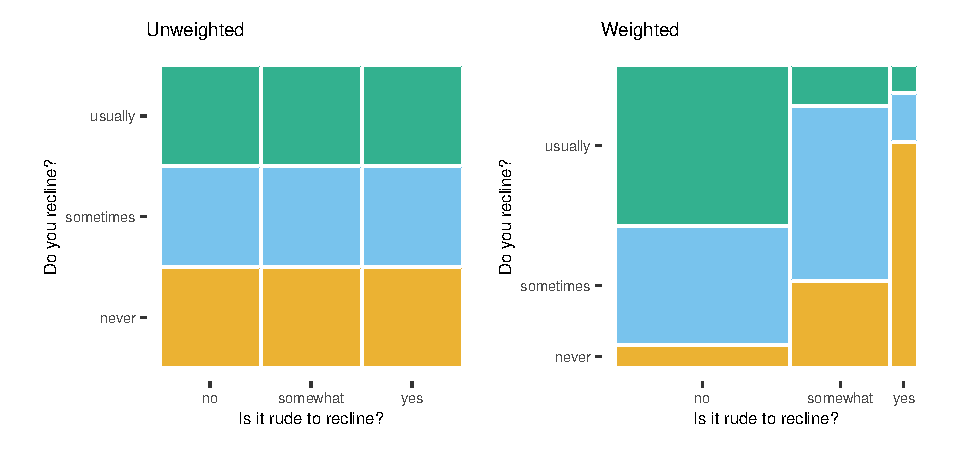
\includegraphics[width=1\linewidth]{RJ-2023-013_files/figure-latex/weight-1} 

}

\caption{When using summarized data, a weighting aesthetic must be defined for the resulting mosaic plot to remain a faithful representation of the data. The mosaic plot on the left contains nine equally sized tiles for the nine combinations that result from the three levels of \code{rude\_to\_recline} crossed with the three levels of \code{do\_you\_recline}. The mosaic plot on the right considers the frequency of those nine combinations resulting in nine tiles proportional to the number of observations each tile represents.}\label{fig:weight}
\end{figure}

The \texttt{weight} aesthetic is also necessary with weighted data, such as weighted surveys. Otherwise, the resulting mosaic plot may not be a faithful representation of the relationship in the data. Here, weights serve to correct imbalances between the sample and the population.

\hypertarget{the-ordering-of-the-variables}{%
\subsubsection{The ordering of the variables}\label{the-ordering-of-the-variables}}

Because of a mosaic plot's hierarchical construction, the ordering of the variables in the formula is vital. While any order of the variables ultimately represents the same data, different variable orders may better support different comparisons. Ideally, the comparison of interest is positioned along a common scale, an easier perceptual task than comparing areas (Cleveland and McGill 1984). In the simple case of two variables, with one an explanatory variable and the other considered the response, the explanatory variable is best placed on the first split of the mosaic and the response variable as the last split, those that occur within each of the tiles created by the first split. The code below and corresponding mosaic plots in Figure \ref{fig:order} illustrate the change that occurs when the variables in the formula are swapped.

\begin{verbatim}
# original order
ggplot(data = flights) +
geom_mosaic(aes(x = product(do_you_recline, rude_to_recline), 
                fill = do_you_recline))

# order reversed
ggplot(data = flights) +
  geom_mosaic(aes(x = product(rude_to_recline, do_you_recline), 
                  fill = do_you_recline))
\end{verbatim}

\begin{figure}

{\centering 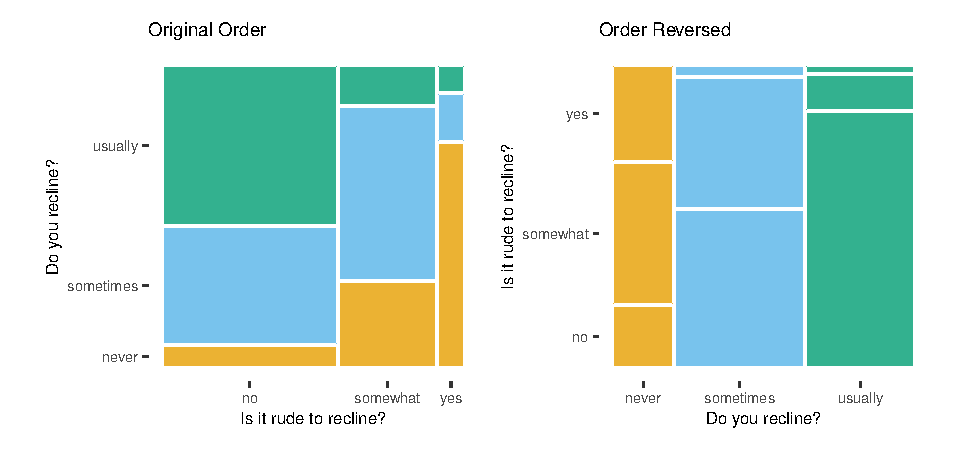
\includegraphics[width=1\linewidth]{RJ-2023-013_files/figure-latex/order-1} 

}

\caption{While the mosaics represent the same data, each supports different comparisons. The mosaic plot on the left emphasizes the effect \code{rude\_to\_recline} has on \code{do\_you\_recline}. The variable order was reversed in the construction of the mosaic plot on the right resulting in a plot that emphasizes the effect \code{do\_you\_recline} has on \code{rude\_to\_recline}.}\label{fig:order}
\end{figure}

The mosaic plots in Figure \ref{fig:order} represent the same joint distribution but are composed differently. The original order, the plot on the left, shows that most of those who believe it is rude to recline never recline their own seat. With the reversed order, we can see that of those who never recline their seats, a roughly equal proportion consider reclining rude as those that do not. The difference highlights how mosaic plots are more than a visualization of the joint distribution; mosaic plots are a visualization of the product of the conditional distribution and marginal distribution, which results in the joint distribution.

In the original order, \texttt{x\ =} \texttt{product(do\_you\_recline,} \texttt{rude\_to\_recline)}, the joint distribution is the product of the conditional distribution of \texttt{do\_you\_recline} given \texttt{rude\_to\_recline} and the marginal distribution of \texttt{rude\_to\_recline}. With this order, we can address questions regarding the marginal distribution of \texttt{rude\_to\_recline}, such as ``what proportion of respondents believe it is rude to recline?'', and questions regarding the conditional distribution of \texttt{do\_you\_recline} given each response to \texttt{rude\_to\_recline}, such as ``Is there an association between a passenger's reclining tendencies and their opinion reclining.

In contrast, \texttt{x\ =} \texttt{product(rude\_to\_recline,} \texttt{do\_you\_recline)}, while resulting in the same joint distribution, is the product of the conditional distribution of \texttt{rude\_to\_recline} given \texttt{do\_you\_recline} and the marginal distribution of \texttt{do\_you\_recline}. Here, we can compare the responses to \texttt{rude\_to\_recline} within each response to \texttt{do\_you\_recline}, which reveals an interesting relationship between a passenger's perceived rudeness given their own inclination to recline. We can see that those that usually recline their seats are more likely to not find reclining to be a rude behavior. Those that never recline their seats, however, are evenly divided with their opinions on reclining. While it is easier to estimate the proportion that never reclines in the reversed order, it is more challenging to decipher what proportion of the respondents believe it is rude to recline, an artifact of the plot representing \texttt{rude\_to\_recline} only through its conditional distribution given the responses to \texttt{do\_you\_recline}.

Ultimately, the preferred order of the variables depends on the comparisons of interest. To (re)arrange the categories within a variable, the levels of the factor variable must be reordered before using \pkg{ggmosaic}.

\hypertarget{the-conds-aesthetic}{%
\subsubsection{\texorpdfstring{The \texttt{conds} aesthetic}{The conds aesthetic}}\label{the-conds-aesthetic}}

The formula setup of the plot can be further altered by electing to view a conditional distribution rather than the full joint distribution. Conditioning can be used to better focus on the comparison of interest either by removing relationships that are not of interest or positioning the comparison of interest along a common scale (Wickham and Hofmann 2011; Cleveland and McGill 1984). When a variable is mapped to the \texttt{conds} aesthetic, the mosaic plot is no longer represents the joint distribution, but instead maps the conditional distribution.

Faceting splits the data into subsets and generates a plot for each subset. Faceting therefore provides another method to accomplish conditioning. The result is the same as with the \texttt{conds} aesthetic, but the formatting is altered. The formatting difference will be discussed in more detail later. Figure \ref{fig:conds} contains an example of each method of conditioning and is based on the code below.

\begin{verbatim}
# not conditioned
ggplot(data = flights) +
  geom_mosaic(aes(x = product(rude_to_recline), 
                  fill = do_you_recline))

# conditioned with aesthetic mapping
ggplot(data = flights) +
  geom_mosaic(aes(x = product(do_you_recline), 
                  fill = do_you_recline, 
                  conds = product(rude_to_recline)))

# conditioned with facets
ggplot(data = flights) +
  geom_mosaic(aes(x = product(do_you_recline), 
                  fill = do_you_recline)) +
  facet_grid(cols = vars(rude_to_recline))
\end{verbatim}

\begin{figure}

{\centering 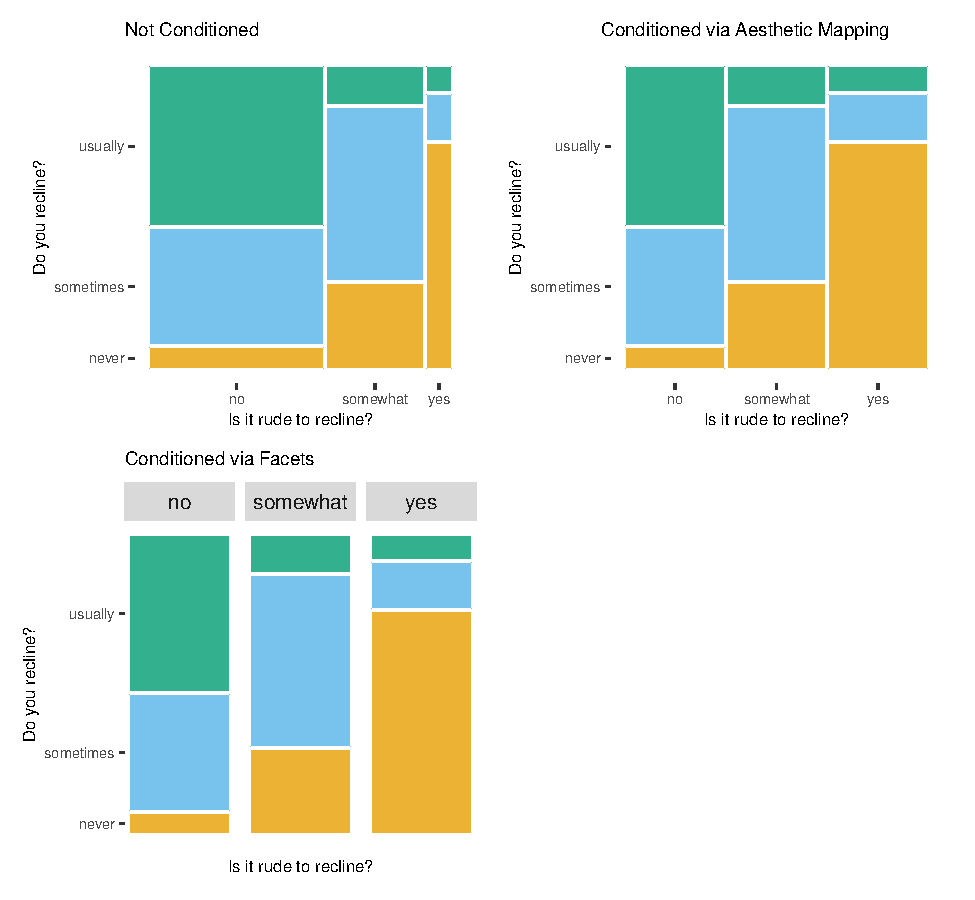
\includegraphics[width=1\linewidth]{RJ-2023-013_files/figure-latex/conds-1} 

}

\caption{Mosaic plots typically depict the joint distribution (top left mosaic plot) but can instead depict the conditional distribution using facetting (bottom left mosaic plot) or the `conds` aesthetic (top right mosaic plot). Conditioning on \code{rude\_to\_recline} may provide a clearer view of the relationship the responses to \code{do\_you\_recline} has with \code{rude\_to\_recline}. However, we lose information on the marginal distribution of \code{rude\_to\_recline}, and the area of a tile is only comparable to the other tiles within that same level of \code{rude\_to\_recline}.}\label{fig:conds}
\end{figure}

For two variables, as in Figure \ref{fig:conds}, the difference between conditioning and not conditioning amounts to the difference between a mosaic plot and a stacked bar chart with a standardized height of 1. That is, when conditioning on \texttt{rude\_to\_recline}, the plot no longer represents the marginal distribution of \texttt{rude\_to\_recline}. Instead, as in a stacked bar chart, the plot only represents the conditional distribution of \texttt{do\_you\_recline} given the responses to \texttt{rude\_to\_recline}.

In the case of three variables, relationships can be removed via conditioning to focus on one relationship in particular and position that relationship along a common scale (Wickham and Hofmann 2011). Figure \ref{fig:conds3} provides an example of conditioning used to focus on the conditional distribution of \texttt{eliminate\_reclining} by removing the joint distribution of \texttt{do\_you\_recline} and \texttt{rude\_to\_recline}. The example is based on the code below.

\begin{verbatim}
# not conditioned
ggplot(flights) +
  geom_mosaic(aes(x = product(eliminate_reclining, do_you_recline,
                              rude_to_recline), 
                  fill = do_you_recline, 
                  alpha = eliminate_reclining))

# conditioned 
ggplot(data = flights) +
  geom_mosaic(aes(x = product(eliminate_reclining), 
                  conds = product(do_you_recline, rude_to_recline), 
                  fill = do_you_recline, 
                  alpha = eliminate_reclining))
\end{verbatim}

\begin{figure}

{\centering 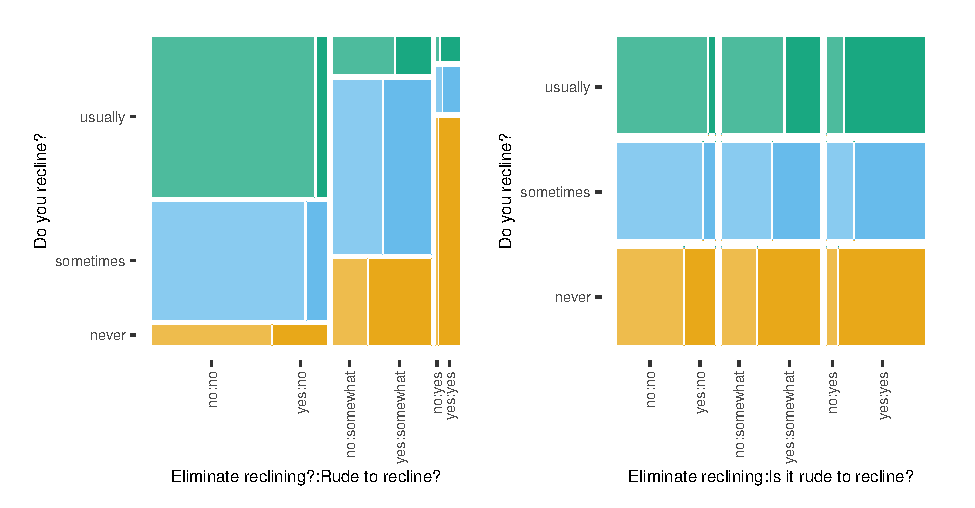
\includegraphics[width=1\linewidth]{RJ-2023-013_files/figure-latex/conds3-1} 

}

\caption{An example of using conditioning to focus on one relationship. The left mosaic plot represents the joint distribution of reclining tendencies, the perceived rudeness of reclining, and the desire to eliminate reclining, providing an overall picture. In the mosaic plot on the right, conditioning on \code{rude\_to\_recline} and \code{do\_you\_recline} removes the representation of the joint distribution of reclining tendencies and the perceived rudeness of reclining but provides a clearer view of the conditional distribution of \code{eliminate\_reclining}.}\label{fig:conds3}
\end{figure}

The conditioning completed in Figure \ref{fig:conds3} provides a better view of how responses to \texttt{eliminate\_reclining} relate to \texttt{do\_you\_recline} and \texttt{rude\_to\_recline} responses. We can see that desires to eliminate reclining are less likely when the respondent reclines their seat. \texttt{eliminate\_reclining} may have a stronger association with responses to \texttt{rude\_to\_recline}, but that comparison is more difficult to make since it is comparing areas rather than positions along a common scale.

When conditioning on multiple variables, it is again important to consider how the variables' order impacts the plot. The two mosaic plots in Figure \ref{fig:conds-orders} display the same data, but the direction of the final split is different. The orientation of the final split determines which comparisons are positioned along a common scale.

\begin{verbatim}
# conditioned order 1
ggplot(data = flights) +
  geom_mosaic(aes(x = product(eliminate_reclining), 
                  conds = product(do_you_recline, rude_to_recline), 
                  fill = do_you_recline, 
                  alpha = eliminate_reclining))

# conditioned order 2
ggplot(data = flights) +
  geom_mosaic(aes(x = product(eliminate_reclining), 
                  conds = product(rude_to_recline, do_you_recline), 
                  fill = do_you_recline, 
                  alpha = eliminate_reclining)) + 
  coord_flip()
\end{verbatim}

\begin{figure}

{\centering 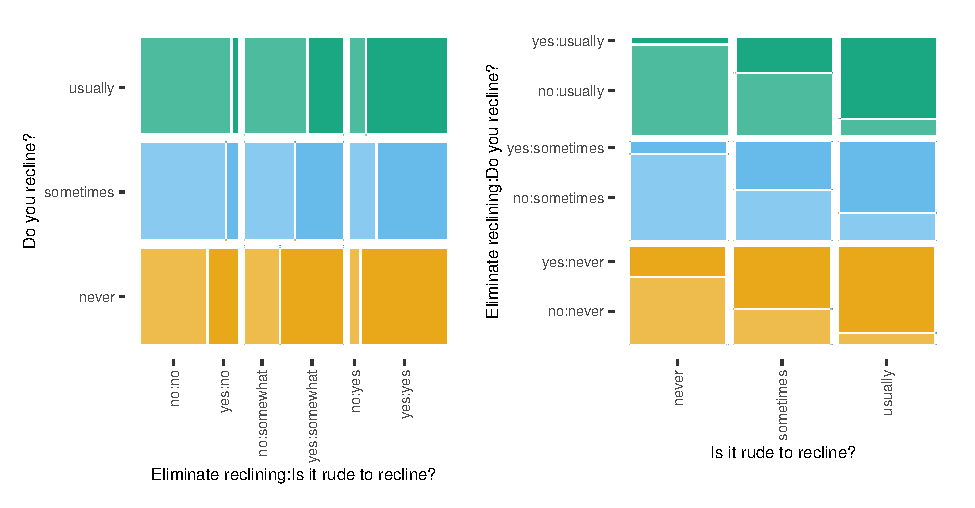
\includegraphics[width=1\linewidth]{RJ-2023-013_files/figure-latex/conds-orders-1} 

}

\caption{The two mosaic plots both portray the distribution of \code{eliminate\_reclining} conditioned on \code{do\_you\_recline} and \code{rude\_to\_recline}, but the direction of the final split is different. The lefthand plot is better suited to compare \code{eliminate\_reclining} with \code{do\_you\_recline}, while the righthand plot is better suited to compare \code{eliminate\_reclining} with \code{rude\_to\_recline}. The comparison of interest should influence the order of the conditioning variables.}\label{fig:conds-orders}
\end{figure}

Figure \ref{fig:conds-orders} rearranges the conditioned variables' order to gauge the strength of the relationship between \texttt{eliminate\_reclining} and \texttt{rude\_to\_recline}. For a fixed level of \texttt{do\_you\_recline}, the desire to eliminate reclining correlates with an increasingly hostile stance on reclining. While this example flips the orders of the conditioned variables and then uses \texttt{coord\_flip()}, \pkg{ggmosaic} provides additional methods of manually modifying the directions of the splits in the mosaic plot, which will be discussed in the next section.

The defined set of aesthetic mappings impacts more than the look of the final graphic; it impacts the analysis and the inquiries the plot can support. \pkg{ggmosaic} requires the \texttt{x} and \texttt{cond} aesthetics to be defined using the \texttt{product()} function to accommodate a variable number of variables. The defined set of aesthetic mappings will result in a model formula that will determine which of the potentially numerous ways the mosaic plot will represent the decomposition of the joint distribution.

\hypertarget{parameters}{%
\subsection{Parameters}\label{parameters}}

Easy customization is necessary for mosaic plots to be effective. Additional aspects of the mosaic plot that can be modified include the strategy used to partition the area into the tiles and the width of the spacing between the tiles. \pkg{ggmosaic} provides the parameters \texttt{divider} and \texttt{offset} to facilitate adjustments to the partitioning strategy and the spacing. This section demonstrates how to create generalized mosaic plots modified by these parameters and how they can be used to highlight different aspects of the data.

In \pkg{ggmosaic}, the desired type of partition is specified with the \texttt{divider} parameter (by setting \texttt{divider\ =\ "\ "}). The area of a mosaic plot can be partitioned into bars or spines, and partitions can be added horizontally or vertically, as shown in Figure \ref{fig:part1} and the code below. When the area is partitioned into bars, the height is proportional to value, and the width equally divides the space. Bars can be arranged horizontally (\texttt{"hbar"}) or vertically (\texttt{"vbar"}). Alternatively, space can be partitioned into spines, where the section's width is proportional to the value, and the height occupies full range. Spines are space-filling and can be arranged horizontally (\texttt{"hspine"}) or vertically (\texttt{"vspine"}). The default divider for a single variable is \texttt{"hspine"}.

\begin{verbatim}
# default / hspine
ggplot(data = flights) + 
  geom_mosaic(aes(x = product(do_you_recline), 
                  fill = do_you_recline))

# vspine
ggplot(data = flights) + 
  geom_mosaic(aes(x = product(do_you_recline), 
                  fill = do_you_recline), 
              divider = "vspine") 

# hbar
ggplot(data = flights) + 
  geom_mosaic(aes(x = product(do_you_recline), 
                  fill = do_you_recline), 
              divider = "hbar") 

# vbar
ggplot(data = flights) + 
  geom_mosaic(aes(x = product(do_you_recline), 
                  fill = do_you_recline), 
              divider = "vbar") 
\end{verbatim}

\begin{figure}[h]

{\centering 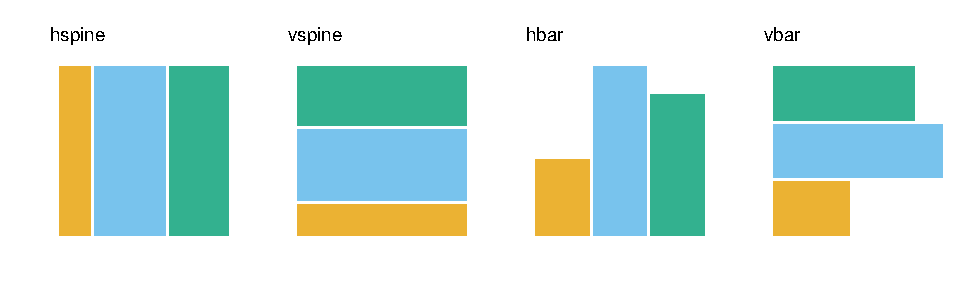
\includegraphics[width=1\linewidth]{RJ-2023-013_files/figure-latex/part1-1} 

}

\caption{Examples of the four ways each dimension in a mosaic plot can be partitioned. While the values are easier to compare with the bars in this one-dimensional example, the advantages of spines become more apparent in higher-dimensional examples.}\label{fig:part1}
\end{figure}

In the case of multiple variables, a type of partition must be defined for each variable. The default divider (\texttt{divider\ =\ mosaic()}) and the double-decker divider (\texttt{divider\ =\ ddecker()}) automatically select a pre-defined pattern for the partitions. For example, if three variables are plotted, the default, \texttt{divider\ =\ mosaic()}, partitions the plot with spines in alternating directions, beginning with a horizontal spine, i.e.~\texttt{divider\ =\ c("hspine",\ "vspine",\ "hspine")}. Alternatively, we can declare the type of partition for each variable, e.g.~\texttt{divider\ =\ c("hbar",\ "vspine",\ "vspine")}. The first partition declared in the vector will be used last in the plot. As mentioned above, an unspecified divider leads to the default \texttt{divider\ =\ mosaic()}, and the partition begins with a horizontal spine and alternate directions for each subsequent variable. To begin with a vertical spine and alternate directions from there, use \texttt{divider\ =\ mosaic(direction\ =\ "v")}. A preview of these options is available in Figure \ref{fig:part3}, and the associated code is below.

\begin{verbatim}
# default / mosaic("h")
ggplot(data = flights) +
  geom_mosaic(aes(x = product(eliminate_reclining, do_you_recline,
                              rude_to_recline), 
                  fill = do_you_recline, 
                  alpha = eliminate_reclining))

# mosaic("v")
ggplot(data = flights) +
  geom_mosaic(aes(x = product(eliminate_reclining, do_you_recline,
                              rude_to_recline), 
                  fill = do_you_recline, 
                  alpha = eliminate_reclining),
              divider = mosaic(direction = "v"))

# ddecker
ggplot(data = flights) + 
  geom_mosaic(aes(x = product(do_you_recline, eliminate_reclining,
                              rude_to_recline), 
                  fill = do_you_recline, 
                  alpha = eliminate_reclining),
              divider = ddecker()) 

# c("hbar", "hbar", "vspine")
ggplot(data = flights) + 
  geom_mosaic(aes(x = product(do_you_recline, rude_to_recline,
                              eliminate_reclining), 
                  fill = do_you_recline, 
                  alpha = eliminate_reclining),
              divider = c("hbar", "hbar", "vspine"))
\end{verbatim}

\begin{figure}

{\centering 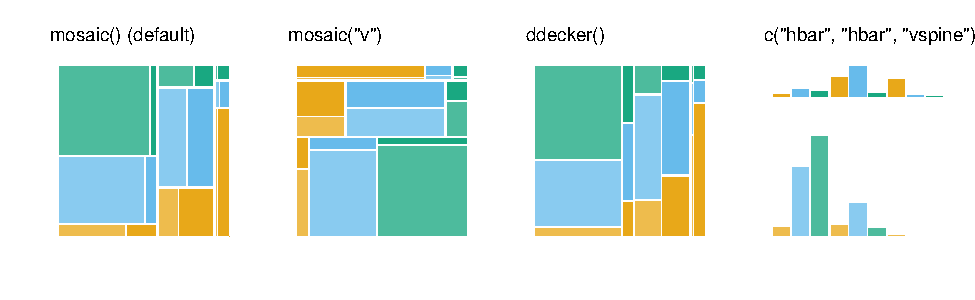
\includegraphics[width=1\linewidth]{RJ-2023-013_files/figure-latex/part3-1} 

}

\caption{When multiple variables are included, a partition type must be defined for each variable, and the different partitions emphasize different relationships. The \code{mosaic()} and \code{ddecker()} functions automatically define a partition for each variable, and are shown in the first and third mosaic plots, respectively. \code{mosaic("v")}, shown in the second plot, is similar to \code{mosaic("h")}, but the coordinates are flipped and inversed. Alternatively, a type of partition can be defined manually for each dimension. \code{ddecker()} emphasizes the conditional distribution of the final variable. In the final plot, the divider \code{c("hbar", "hbar", "vspine")} creates a plot similar to a faceted bar chart that supports comparisons similar to those supported by the double-decker plot but for relative values instead of relative proportions.}\label{fig:part3}
\end{figure}

The \texttt{divider} parameter provides an additional mechanism for modifying the plot's arrangement to focus on a particular relationship by enabling a user to modify any dimension of the divider to position the comparison of interest along a common scale. For instance, the double-decker plot in Figure \ref{fig:part3} helps compare the effects changes in \texttt{eliminate\_reclining} and \texttt{rude\_to\_recline} have on the responses to \texttt{do\_you\_recline} and how the relationship between \texttt{do\_you\_recline} and \texttt{eliminate\_reclining} differs for different levels of \texttt{rude\_to\_recline}.

\pkg{ggmosaic} adopts the procedure followed by Hartigan and Kleiner (1981), Friendly (2002), Theus and Urbanek (2009), and Hofmann (2003), where an amount of space is allocated for each of the splits, with subsequent divisions receiving a smaller amount of space. The splits between the categories of the first variable are the widest and the splits decrease in width with each additional variable. Decreasing the widths of the splits with each additional variable allows the categories to group together according to the recursive strategy (Theus and Urbanek 2009) and the created spaces preserve the impact of small counts (Friendly 2002). The effect becomes apparent when an empty group is included. In this case, the spaces between the empty categories create a gap equal to the amount of space that is between non-empty categories.

For variables with many categories, it may be of interest to decrease the size of the spacing between the spines. The parameter \texttt{offset} can widen or shrink the size of the spacing between the categories of the first variable and the subsequent splits then gradually decrease in width with each additional variable. The default setting of this parameter is \texttt{offset\ =\ 0.01}, equivalent to 1\% of the width of the plotting area. The code below and the corresponding mosaic plots in Figure \ref{fig:space} demonstrate how to use the \texttt{offset} parameter.

\begin{verbatim}
# increased spacing
ggplot(data = flights) +
  geom_mosaic(aes(x = product(rude_to_recline), 
                  fill = do_you_recline),
              offset = 0.03) 
  
# decreased spacing
ggplot(data = flights) +
  geom_mosaic(aes(x = product(rude_to_recline), 
                  fill = do_you_recline),
              offset = 0) 

# default spacing
ggplot(data = flights) +
  geom_mosaic(aes(x = product(rude_to_recline), 
                  fill = do_you_recline)) 
\end{verbatim}

\begin{figure}

{\centering 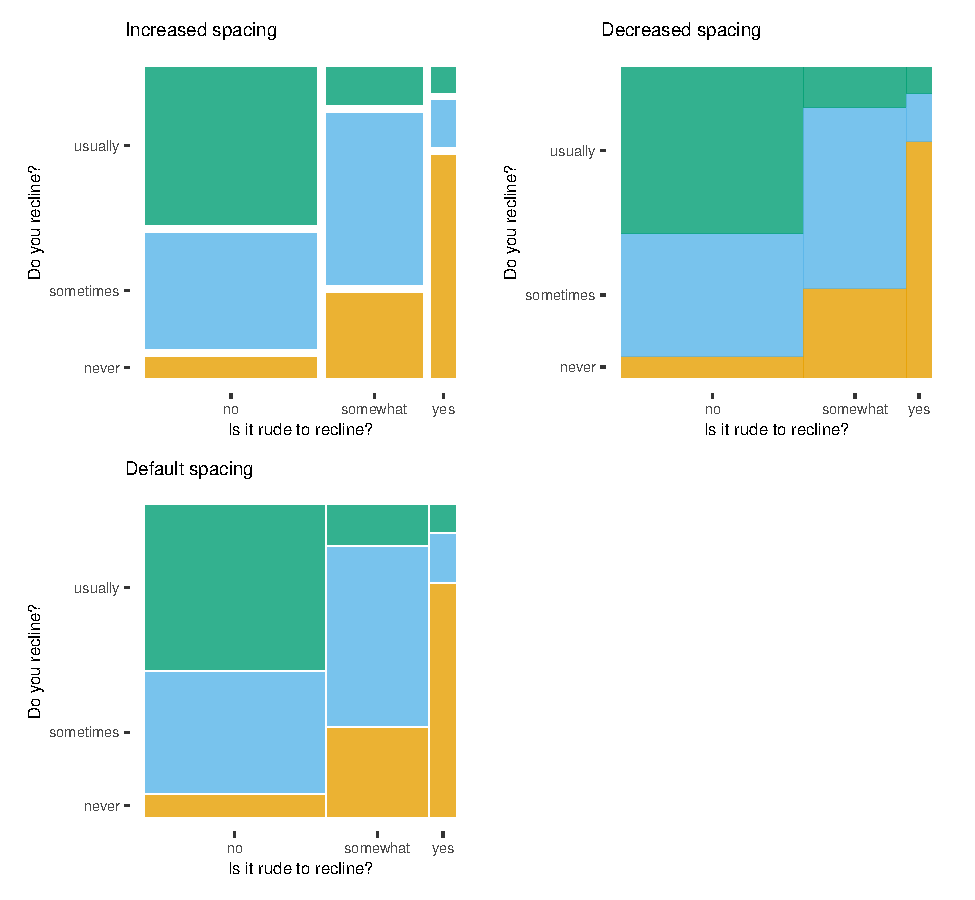
\includegraphics[width=1\linewidth]{RJ-2023-013_files/figure-latex/space-1} 

}

\caption{Three examples of how the spacing of the splits in the mosaic plot can be increased or decreased with the offset parameter.}\label{fig:space}
\end{figure}

While the examples so far include up to three variables, there is no technical limit to the number of variables in a mosaic plot. However, when many categorical variables are present, mosaic plots can quickly become cluttered and difficult to interpret, and a judgment call must be made on the practical limit to the number of variables included in the mosaic plot. This practical limit could depend on many factors, including the number of categories within each variable, the viewing size of the result mosaic plot, and the viewer's familiarity with the data.

The customization offered via the \pkg{ggmosaic} parameters allows users to easily make complex generalized mosaic plots that are more readable and simpler to interpret. The parameters provide additional dimensions of freedom with the ability to switch between bars and spines and allow users to highlight different aspects of high-dimensional categorical data to identify and communicate interesting patterns.

\hypertarget{interactivity}{%
\subsection{Interactivity}\label{interactivity}}

Having a geom designed for generalized mosaic plots allows for a \texttt{ggplotly()} hook to create interactive mosaic plots with the \CRANpkg{plotly} package, version 4.9.3 (Sievert et al. 2016). The \texttt{ggplotly()} function translates most of the basic geoms bundled with the \pkg{ggplot2} package. To expand the functionality to custom geoms, we make use of the infrastructure provided in the \pkg{plotly} package that allows for a translation. In \pkg{ggplot2}, many geoms are special cases of other geoms. For example, \texttt{geom\_line()} is equivalent to \texttt{geom\_path()} once the data is sorted by the \texttt{x} variable. Because \texttt{GeomMosaic} can be reduced to the lower-level geom \texttt{GeomRect}, we were able to write a method for the \texttt{to\_basic()} generic function in \pkg{plotly} (Sievert 2020). Figure \ref{fig:plotly-static} features an example of an interactive mosaic plot created with \texttt{ggplotly()} and the corresponding code is below.

\begin{verbatim}
p1 <- ggplot(data = flights) +
  geom_mosaic(aes(x = product(rude_to_recline), 
                  fill = do_you_recline)) 

plotly::ggplotly(p1)
\end{verbatim}

\begin{figure}

{\centering 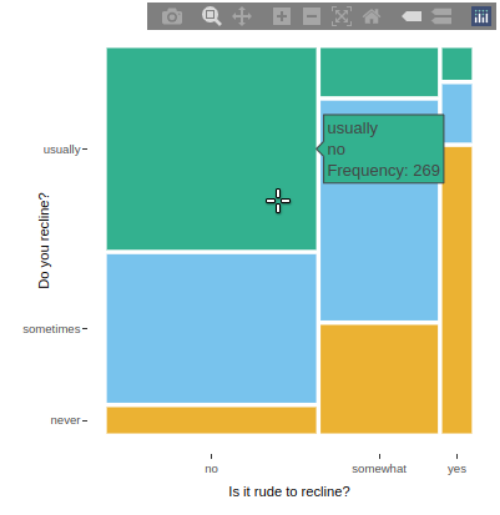
\includegraphics[width=0.6\linewidth]{plotly} 

}

\caption{Users can create interactive mosaic plots using  \pkg{ggmosaic} with \pkg{plotly}. With plotly, users gain the ability to hover over a tile to see the names of the combination of levels and the number of observations that the tile represents.}\label{fig:plotly-static}
\end{figure}

\hypertarget{new-features-in-version-0.3.3}{%
\section{\texorpdfstring{New features in \pkg{ggmosaic} version 0.3.3}{New features in  version 0.3.3}}\label{new-features-in-version-0.3.3}}

The layered grammar implemented by \pkg{ggplot2} provides a means to add additional layers (typically resulting in additional geometric objects) to a graphic. The unique scale system in \pkg{ggmosaic}, however, makes a correct placement of items in additional layers tricky. The \texttt{x} and \texttt{y} scales in a mosaic plot are both numeric and categorical; the numeric scale determines the placement of additional objects on a range between \texttt{0} and \texttt{1}. Thus, to place an object in the center of each tile, it is necessary to know the numeric values for the corners of each of the tiles. Version 0.3.3 of \pkg{ggmosaic} introduced two additional geoms designed to build on \texttt{stat\_mosaic()} and \texttt{geom\_mosaic()} that bypass these calculations.

The two geoms, \texttt{geom\_mosaic\_text()} and \texttt{geom\_mosaic\_jitter()}, are provided to further enhance the generalized mosaic plots created with \pkg{ggmosaic}. These features are designed to add labels to the mosaic plot tiles and to view the tiles' density via jittered points, and are implemented as additional geom items that can layer on top of the original mosaic geom. Lastly, we also provide a new minimal theme, \texttt{theme\_mosaic()}, designed for mosaic plots. The theme removes items from the plot background in order to reduce clutter and increase readability. Together, these features add new functionality to mosaic plots to increase their usability and facilitate more profound insights into high-dimensional categorical data.

\hypertarget{a-labeling-geom}{%
\subsection{A labeling geom}\label{a-labeling-geom}}

The flexibility of generalized mosaic plots can lead to inadequate space around the perimeter of the plot to label each of the categories for the variables displayed, making labeling a challenge. To ease the burden on the axis labels, \texttt{geom\_mosaic\_text()} applies labels to the tiles. This section introduces \texttt{geom\_mosaic\_text()}, its parameters, and its customization options with sample code and graphics.

One aspect of mosaic plots is that while the text and tick marks on the axes may be aligned with the correct category levels on one side of the plot, the alignments may not be appropriate for category levels on the opposite side of the plot. Thus, it may be advantageous to label the tiles to ensure the group identities are apparent to a viewer. \texttt{geom\_mosaic\_text()} provides the means to place text, or labels, in each of the tiles. \texttt{geom\_mosaic\_text()} has its counterpart, \texttt{stat\_mosaic\_text()}, perform the necessary mapping calculations to place each tile's label in the center of the tile. Figure \ref{fig:labels} features an example created with \texttt{geom\_mosaic()} with \texttt{geom\_mosaic\_text()} added to place text in each of the tiles corresponding to the tiles' combination of categories. The associated code is below.

\begin{verbatim}
ggplot(data = flights) +
  geom_mosaic(aes(x = product(do_you_recline, rude_to_recline), 
                  fill = do_you_recline)) +
  geom_mosaic_text(aes(x = product(do_you_recline, rude_to_recline)))
\end{verbatim}

\begin{figure}[h]

{\centering 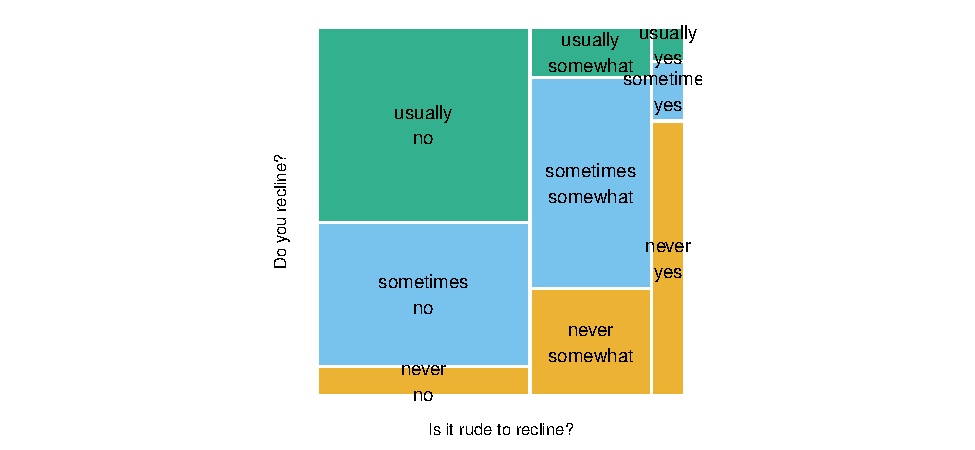
\includegraphics[width=1\linewidth]{RJ-2023-013_files/figure-latex/labels-1} 

}

\caption{In this example, a geom of labels is layered on top of the mosaic geom to produce a mosaic plot with labels centered in each tile. Directly labeling each tile can alleviate issues caused by inadequate space around the perimeter for labels.}\label{fig:labels}
\end{figure}

As a default, the label text contains the combinations of category levels the tile represents. Alternative labels may be desired and are achievable through the \texttt{label} aesthetic. For example, to label the tiles of a mosaic with counts, that variable can be mapped to the \texttt{label} aesthetic. The counts, however, need not be contained in the underlying data before plotting; the function \texttt{after\_stat()} supports aesthetic mappings of variables calculated by the stat, in this case, the variable \texttt{.wt} calculated in \texttt{stat\_mosaic\_label()} (see Figure \ref{fig:labels2} and the code below).

\begin{verbatim}
ggplot(data = flights) +
  geom_mosaic(aes(x = product(do_you_recline, rude_to_recline), 
                  fill = do_you_recline)) +
  geom_mosaic_text(aes(x = product(do_you_recline, rude_to_recline), 
                       label = after_stat(.wt)))
\end{verbatim}

\begin{figure}

{\centering 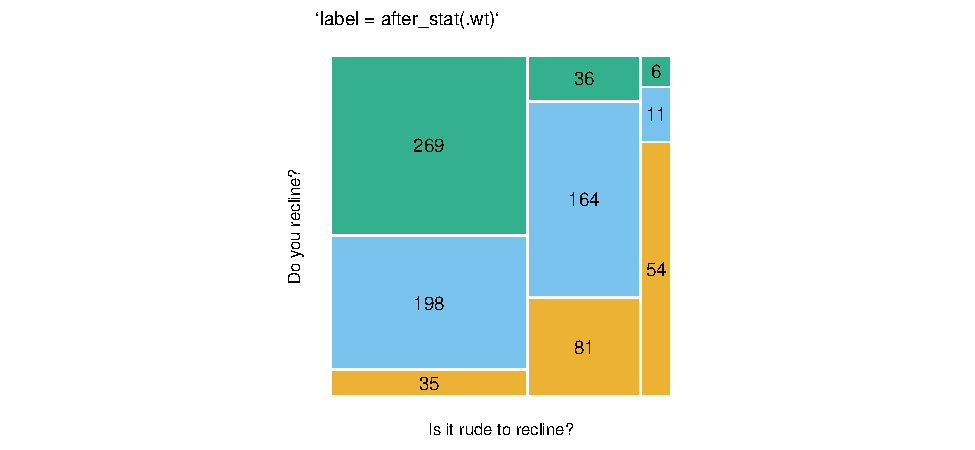
\includegraphics[width=1\linewidth]{RJ-2023-013_files/figure-latex/labels2-1} 

}

\caption{Variables calculated by the associated stat can be used for the label. In this example, \code{.wt} is used to place the frequencies represented by the tile in the center of that tile, providing a glance at the size of the data and removing potential guessing work aimed at comparing areas of unaligned tiles.}\label{fig:labels2}
\end{figure}

To help label the areas of the plots where labels may be densely packed and overlapping, \pkg{ggmosaic} uses the \pkg{ggplot2} extension package, \CRANpkg{ggrepel} (Slowikowski 2021). The geoms provided by ggrepel help ensure the text is readable by repelling the labels away from each other, data points, and edges of the plot panel. In addition to the standard \texttt{"Text"} and \texttt{"Label"} geoms, \pkg{ggmosaic}'s use of \pkg{ggrepel} allows the use of the \texttt{"TextRepel"} and \texttt{"LabelRepel"} geoms within mosaic plots. Thus, \texttt{geom\_mosaic\_text()} provides access to the features of four geoms. To access these four geoms, the parameters \texttt{as.label} and \texttt{repel} are introduced; their use is demonstrated in Figure \ref{fig:label-opts}, and the code is below. Furthermore, the parameter \texttt{repel\_params} is available to use with either of the \pkg{ggrepel} options, and the parameter \texttt{check\_overlap} is available to use with the \texttt{"Text"} geom.

\begin{verbatim}
# default / text
ggplot(data = flights) +
  geom_mosaic(aes(x = product(do_you_recline, rude_to_recline), 
                  fill = do_you_recline)) +
  geom_mosaic_text(aes(x = product(do_you_recline, rude_to_recline)))

# label
ggplot(data = flights) +
  geom_mosaic(aes(x = product(do_you_recline, rude_to_recline), 
                  fill = do_you_recline)) +
  geom_mosaic_text(aes(x = product(do_you_recline, rude_to_recline)), 
                   as.label = TRUE)
  
# repel text
ggplot(data = flights) +
  geom_mosaic(aes(x = product(do_you_recline, rude_to_recline), 
                  fill = do_you_recline)) +
  geom_mosaic_text(aes(x = product(do_you_recline, rude_to_recline)), 
                   repel = TRUE)
  
# repel label
ggplot(data = flights) +
  geom_mosaic(aes(x = product(do_you_recline, rude_to_recline),
                  fill = do_you_recline)) +
  geom_mosaic_text(aes(x = product(do_you_recline, rude_to_recline)), 
                   repel = TRUE, as.label = TRUE)
\end{verbatim}

\begin{figure}

{\centering 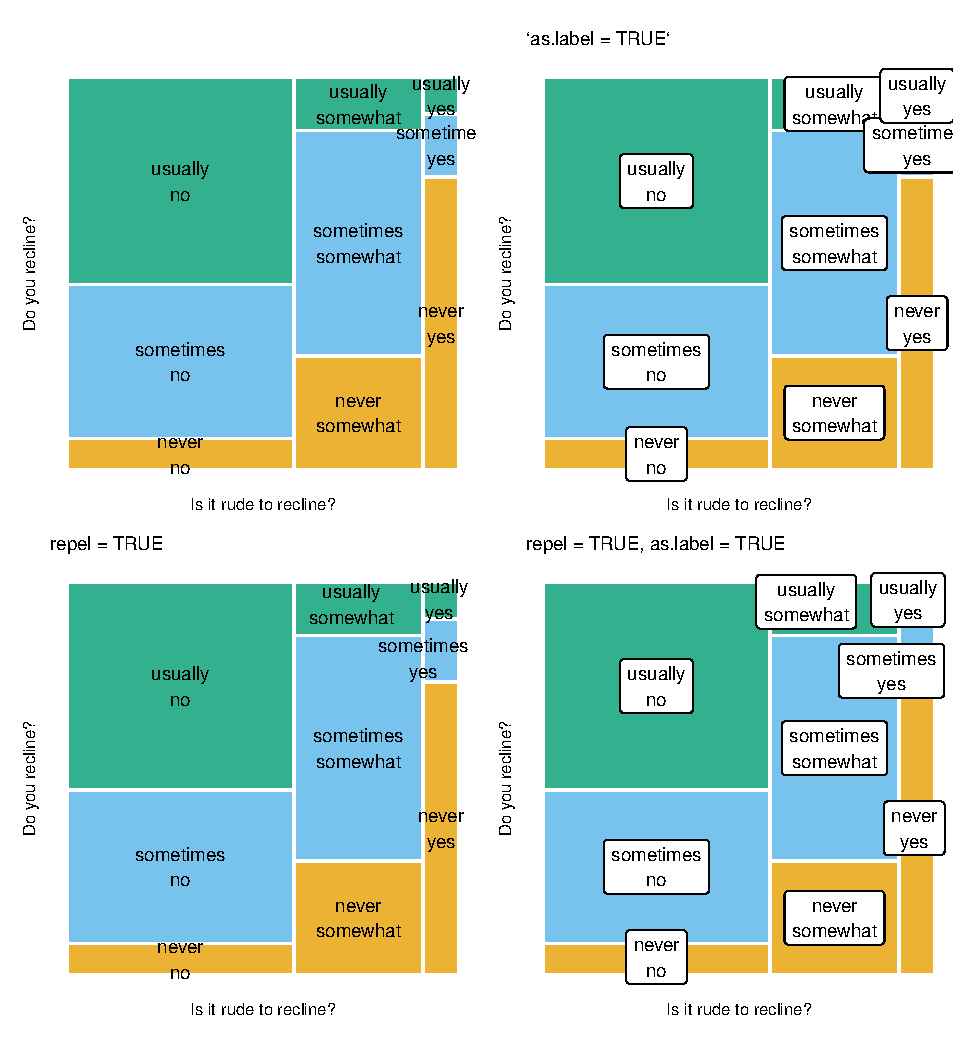
\includegraphics[width=1\linewidth]{RJ-2023-013_files/figure-latex/label-opts-1} 

}

\caption{Examples of the four geoms accessible to \code{geom\_mosaic\_text()}. The geoms, from left to right and top to bottom, are \code{"Text"}, \code{"Label"}, \code{"TextRepel"}, and \code{"LabelRepel"}.}\label{fig:label-opts}
\end{figure}

Mosaic plots with many categories can quickly become unreadable, \texttt{geom\_mosaic\_text()} helps alleviate congestion-related confusion by providing quick and effective labeling in various formats. The parameters \texttt{repel} and \texttt{as.label} provide access to three additional geoms. The geom \texttt{geom\_mosaic\_text()} can add the text geom, the label geom, the \pkg{ggrepel} text geom, or the \pkg{ggrepel} label geom. The parameters \texttt{repel\_params} and \texttt{check\_overlap} provide access to the parameters native to the \pkg{ggrepel} geoms and label geoms, respectively. Labels add value to the mosaic plot as they ensure easy and correct identification of the tiles, which, in turn, eases the visual analysis.

\hypertarget{a-jittering-geom}{%
\subsection{A jittering geom}\label{a-jittering-geom}}

In constructing of a mosaic plot, the tile area is proportional to the number of observations that the tile represents. In other words, the density of each tile in a mosaic plot is constant throughout the plot. While the number of observations, or density, is typically masked in a mosaic plot, a user can visualize these individual data points with \texttt{geom\_mosaic\_jitter()}. This added layer of visualization unlocks a range of applications, from adding additional aesthetic mappings, both included in the formula and not, to model diagnosis. Research suggests visualizations that incorporate individuals in charts allow viewers to digest and understand probabilities and risks involved more easily (Galesic, Garcia-Retamero, and Gigerenzer 2009; Ancker et al. 2006). These features further extend the ability of generalized mosaic plots to communicate interesting features of high-dimensional categorical data.

When used in conjunction with \texttt{geom\_mosaic()}, \texttt{geom\_mosaic\_jitter()} adds a layer of jittered points superimposed on the mosaic plot. The number of points in each rectangle is equal to the number of observations that the rectangle represents. The result is an even dispersal of points throughout the one-by-one square mosaic plot.

When conditioning on a variable, \texttt{geom\_mosaic\_jitter()} provides a visual representation of the differences between the conditional probability and the joint probability; the spread of the points throughout the mosaic plot can help decipher a conditioning variable's effect on a mosaic plot's construction. In Figure \ref{fig:jitter}, conditioning on the variable \texttt{rude\_to\_recline} causes a change in the density of the jittered points. The visual difference serves as an effective tool for teaching the concept. The plots are based on the following lines of code:

\begin{verbatim}
# not conditioned
ggplot(data = flights) +
  geom_mosaic(aes(x = product(rude_to_recline), 
                  fill = do_you_recline), 
              alpha = 0.3) +
  geom_mosaic_jitter(aes(x = product(rude_to_recline), 
                         color = do_you_recline))
  
# conditioned
ggplot(data = flights) +
  geom_mosaic(aes(x = product(do_you_recline), 
                  conds = product(rude_to_recline), 
                  fill = do_you_recline), 
              alpha = 0.3)  +
  geom_mosaic_jitter(aes(x = product(do_you_recline), 
                         conds = product(rude_to_recline), 
                         color = do_you_recline))
\end{verbatim}

\begin{figure}[h]

{\centering 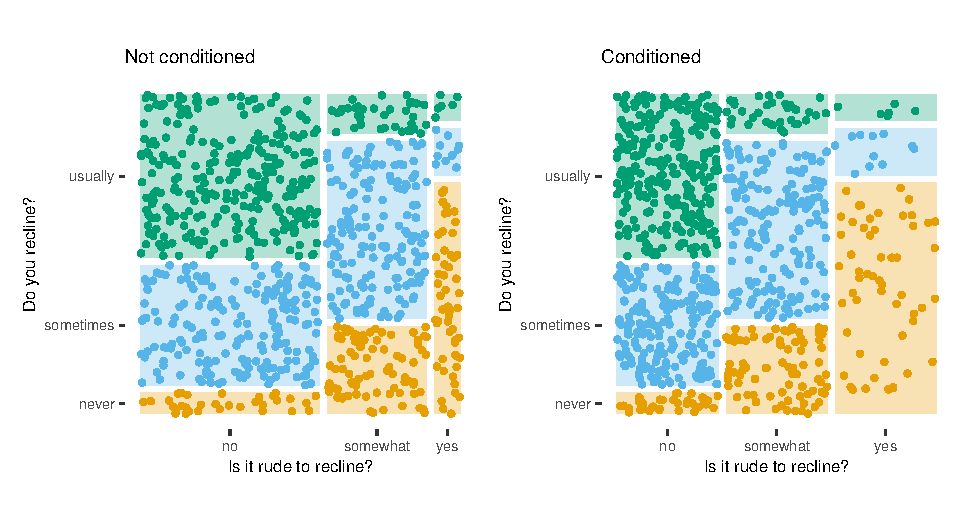
\includegraphics[width=1\linewidth]{RJ-2023-013_files/figure-latex/jitter-1} 

}

\caption{This example highlights the differences between the conditional (right) and joint (left) probability with the density of the jittered dots. When conditioning, the columns are equally sized, and the jittered points condense into the leftmost column, previously the widest column, rather than being evenly dispersed.}\label{fig:jitter}
\end{figure}

Including the jittered points generates an awareness of the size of the data, something customarily masked in a mosaic plot. For smaller data sets such as the \texttt{titanic} data set, using \texttt{geom\_mosaic\_jitter()} may encourage engagement as the points connect with the individuals in the data. This connection may provide a more compelling and profound visual impact.

\texttt{geom\_mosaic\_jitter()} is more effective when the \texttt{alpha} argument is used in both \texttt{geom\_mosaic\_jitter()} and \texttt{geom\_mosaic()} to create semi-transparent jittered points and semi-transparent rectangles. An \texttt{alpha} value of \texttt{0.3} for \texttt{geom\_mosaic()} and an \texttt{alpha} value of \texttt{0.7} for \texttt{geom\_mosaic\_jitter()} is aesthetically pleasing.

\texttt{geom\_mosaic\_jitter()} introduces an additional parameter, \texttt{drop\_level}. The \texttt{drop\_level} parameter controls which level defines the color of the generated points. In other words, if a \texttt{color} aesthetic is defined, should that variable be included in the formula? If the formula includes the \texttt{color} aesthetic, \texttt{drop\_level\ =\ FALSE}, the colored points are at the top level. If the formula does not include the \texttt{color} aesthetic, \texttt{drop\_level\ =\ TRUE}, color is added to the points one level down. Figure \ref{fig:leveldown} provides an example of these two options.

\begin{verbatim}
# drop level
ggplot(data = flights) +
  geom_mosaic(aes(x = product(rude_to_recline)), 
              alpha = 0.1) +
  geom_mosaic_jitter(aes(x = product(rude_to_recline), 
                         color = do_you_recline),
                     drop_level = TRUE)
# do not drop level
ggplot(data = flights) +
  geom_mosaic(aes(x = product(rude_to_recline)), 
              alpha = 0.1) +
  geom_mosaic_jitter(aes(x = product(rude_to_recline), 
                         color = do_you_recline),
                     drop_level = FALSE)
\end{verbatim}

\begin{figure}

{\centering 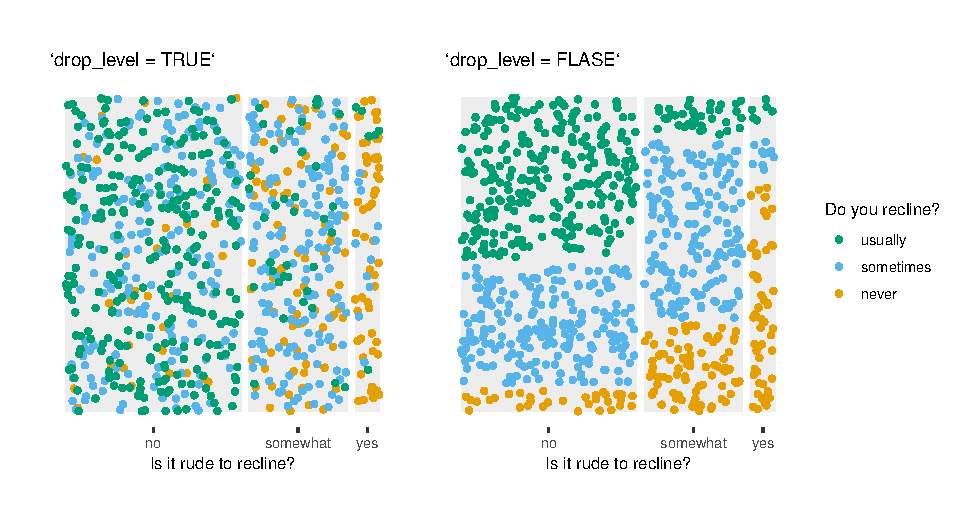
\includegraphics[width=1\linewidth]{RJ-2023-013_files/figure-latex/leveldown-1} 

}

\caption{The parameter \code{drop\_level} controls which level defines the colors of the generated points. On the left, color is added to the points one level down, and a mixing of the colored points occurs. In the plot on the right, the heights of the sorted points' spaces represent the conditional distribution of \code{do\_you\_recline} given \code{rude\_to\_recline}. }\label{fig:leveldown}
\end{figure}

An additional aesthetic, \texttt{weight2}, is implemented in \texttt{geom\_mosaic\_jitter()}. The \texttt{weight2} aesthetic allows the number of points generated within each tile to be different from the number of points the cell represents.

While mosaic plots are typically drawn according to the observed values, they can be drawn according to the model's expected values.

\begin{verbatim}
flights_model %>% glimpse()
\end{verbatim}

\begin{verbatim}
#> Rows: 9
#> Columns: 4
#> $ do_you_recline  <fct> never, never, never, sometimes, sometimes, sometimes, ~
#> $ rude_to_recline <fct> no, somewhat, yes, no, somewhat, yes, no, somewhat, yes
#> $ Observed        <int> 35, 81, 54, 198, 164, 11, 269, 36, 6
#> $ Expected        <dbl> 100, 56, 14, 219, 123, 31, 183, 102, 26
\end{verbatim}

Figure \ref{fig:model} displays the observed values on the left and the expected values from the independence model on the right. The difference between the two plots represents the lack of fit. The plot is based on the following lines of code:

\begin{verbatim}
flights_model %>% 
  gather("wt_type", "wt", Expected:Observed) %>% 
  ggplot() + 
  geom_mosaic(aes(weight = wt, 
                  x = product(rude_to_recline), 
                  fill = do_you_recline)) +
  facet_wrap(vars(wt_type))
\end{verbatim}

\begin{figure}[h]

{\centering 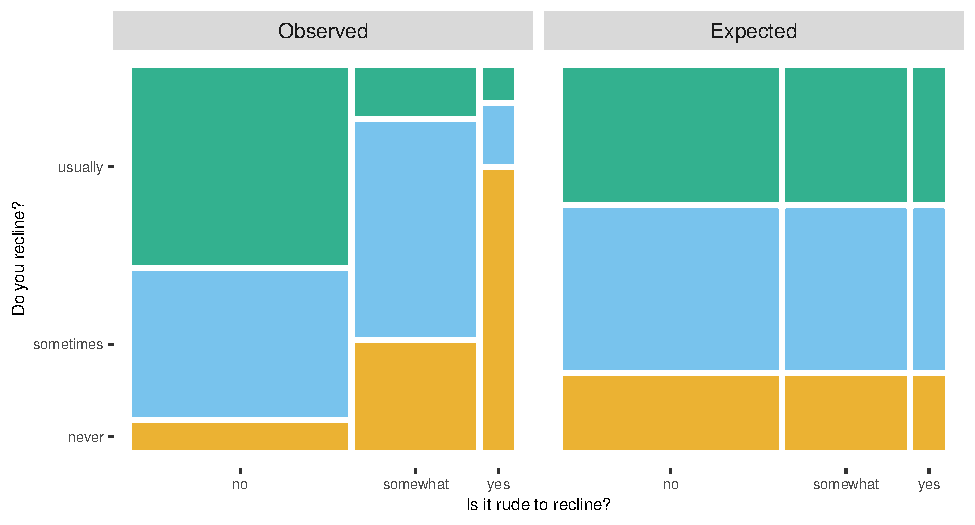
\includegraphics[width=1\linewidth]{RJ-2023-013_files/figure-latex/model-1} 

}

\caption{While mosaic plots are typically drawn according to the observed values, they can be drawn according to the model's expected values. The mosaic plot on the right displays the expected values from the independence model, recognizable by the lattice structure. The differences in the heights of the tiles in the observed data mosaic plot on the left reveal a strong association between the two variables, and the differences between the two plots highlight the lack of model fit.}\label{fig:model}
\end{figure}

In Figure \ref{fig:model}, the mosaic plot drawn according to the observed values represents the data space, whereas the mosaic plot drawn according to the expected values represents the model space. Rather than requiring two plots, jittering connects in one plot both the data space with the model space highlighting the differences between the two.

In Figure \ref{fig:weight2}, the jittered points represent the observed values, while the tiles' size represents the expected values. We can evaluate the fit of the model according to how evenly the points spread throughout the plot. For example, the overcrowded points seen in the leftmost bottom tile communicate that the independence model underestimates the number of respondents that think it is rude to recline and never recline their seats.

\begin{verbatim}
ggplot(flights_model) + 
  geom_mosaic(aes(weight = Expected, 
                  x = product(do_you_recline, rude_to_recline)), 
              alpha = .2) +
  geom_mosaic_jitter(aes(weight2 = Observed, 
                         weight = Expected, 
                         x = product(do_you_recline, rude_to_recline)))
\end{verbatim}

\begin{figure}

{\centering 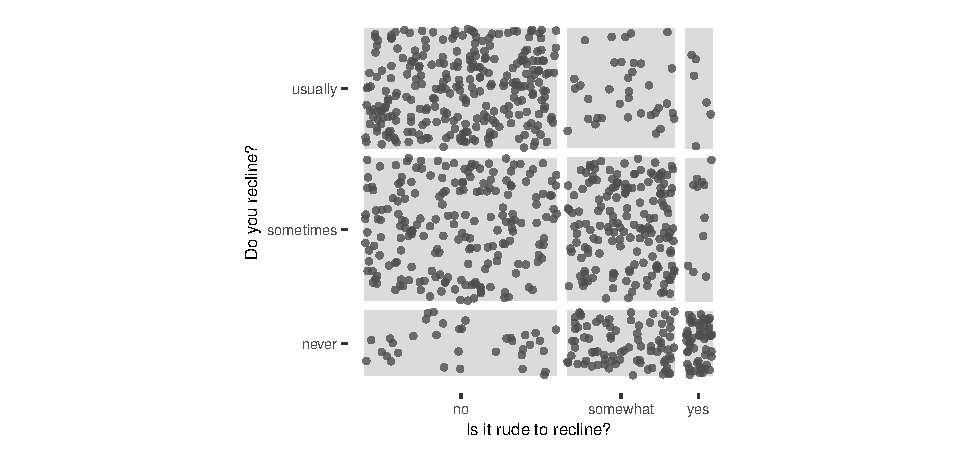
\includegraphics[width=1\linewidth]{RJ-2023-013_files/figure-latex/weight2-1} 

}

\caption{In this example, the tiles of the mosaic plot are drawn according to the expected values. A jitter geom representing the observed values is layered on top. The uneven dispersal of the points indicates a lack of fit.}\label{fig:weight2}
\end{figure}

The jitter geom, with its additional aesthetic mappings, provides a convenient visual aide that can help solidify what the mosaic plot represents and help communicate the differences between conditional and joint probabilities. The implementation of the jitter geom allows the user to extend the functionality of mosaic plots beyond what has previously been available.

\hypertarget{a-custom-theme}{%
\subsection{A custom theme}\label{a-custom-theme}}

Mosaic plots have two main characteristics that set mosaic plots apart from other graphics. First, at its foundation, a mosaic plot is a one-by-one square, and the area of each tile in the mosaic plot is proportional to the frequency of the combination of categories that the tile represents. Second, mosaic plots do not have a standard coordinate system. Rather, mosaic plots have a coordinate system based on recursive partitioning that can integrate several variables. These two characteristics clash with the default \pkg{ggplot2} theme. For this reason, version 0.3.3 of \pkg{ggmosaic} includes a custom theme for mosaic plots, \texttt{theme\_mosaic()}, that can be added to the plot in the same manner as any other \pkg{ggplot2} theme. (Figure \ref{fig:themes})

The plot grid lines suffer from the same issue as the axis labels; while the grid lines may be aligned with the
correct category levels on one side of the plot, the alignments may not be appropriate for category levels on the opposite side of the plot. \texttt{theme\_mosaic()} removes all grid lines but does not remove the axis labels and ticks.

Seeking a more faithful representation of a mosaic plot, \texttt{theme\_mosaic()} enforces a fixed aspect ratio of 1. When faceting, the aspect ratio should be modified according to the number of panels and the direction of the faceting. For example, in Figure \ref{fig:aspect}, the faceting represents the responses to \texttt{do\_you\_recline} conditioned on the responses to \texttt{rude\_to\_recline}. The conditioning variable, \texttt{rude\_to\_recline}, contains three categories, and the faceting represents a horizontal spine. Hence, the aspect ratio is modified from \texttt{1} (the default) to \texttt{3}.

\begin{figure}

{\centering 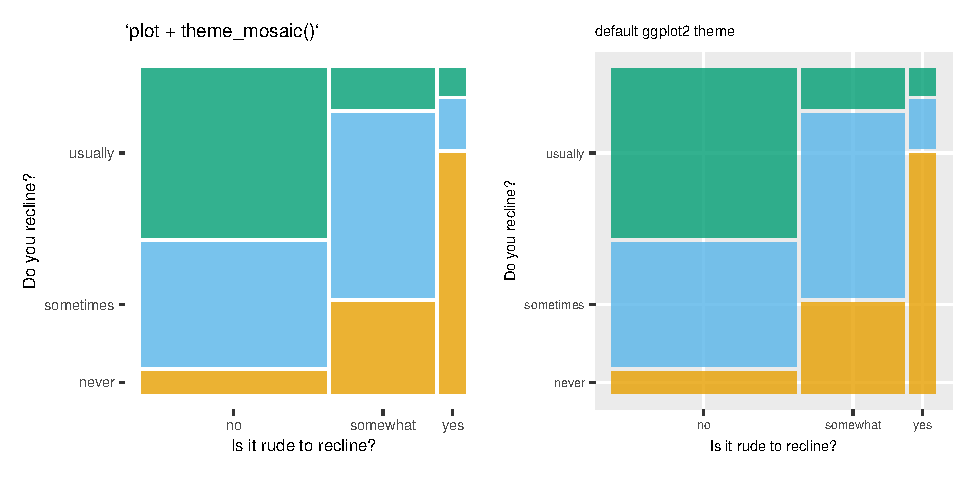
\includegraphics[width=1\linewidth]{RJ-2023-013_files/figure-latex/themes-1} 

}

\caption{This example highlights the differences between the custom theme (left) and the default theme (right). The custom theme for mosaic plots seeks to minimize clutter by removing the plot background and the grid lines.}\label{fig:themes}
\end{figure}

\begin{figure}

{\centering 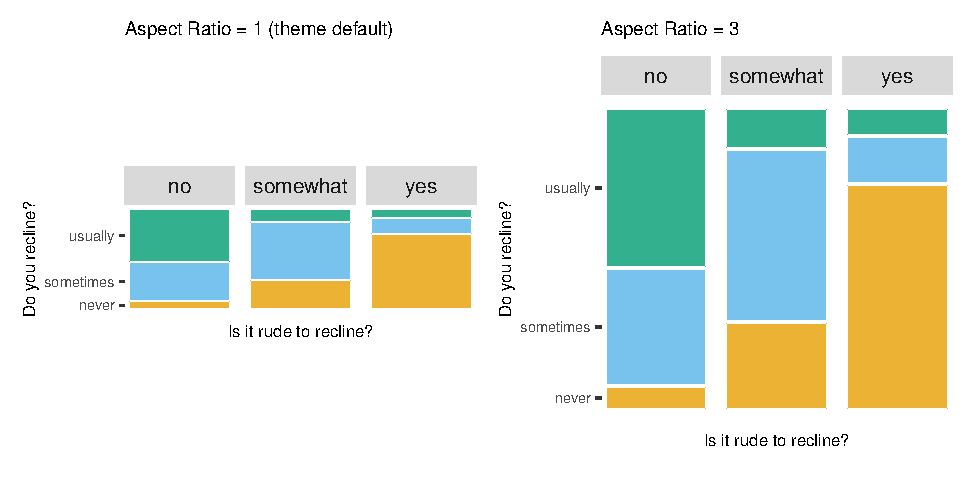
\includegraphics[width=1\linewidth]{RJ-2023-013_files/figure-latex/aspect-1} 

}

\caption{When using faceting, the aspect ratio might need to be adjusted according to the desired outcome. The default (left) represents each facet as a 1-by-1 mosaic plot, whereas an aspect ratio of 3 (right) represents each facet as one equal-sized column within a 1-by-1 mosaic plot.}\label{fig:aspect}
\end{figure}

The custom theme, \texttt{theme\_mosaic()}, seeks to help a viewer extract the correct information from the plot by providing a more suitable default aspect ratio and removing the axes lines that are not always appropriate across the entire plot. As with any theme, however, \texttt{theme\_mosaic()} is merely a suggestion of a starting-off point, and it can be modified as seen fit for each individual plot.

\hypertarget{interactive-exploratory-mosaic-plot-building}{%
\section{Interactive exploratory mosaic plot building}\label{interactive-exploratory-mosaic-plot-building}}

Mosaic plots help identify interesting relationships in high-dimensional categorical data and are an influential tool for exploratory data analysis (EDA). Because of the complexities that arise from comparing many categories, it is often necessary to iterate through many of the potential mosaic plots and obtain many views on the data. The addition of interactivity to the generation of mosaic plots can ease this process and help mosaic plots become more valuable and insightful (Hofmann 2003).

To facilitate exploring data with mosaic plots, \pkg{ggmosaic} version 0.3.4 includes a Shiny application that can be launched with the function \texttt{ggmosaic\_app()} (Figure \ref{fig:app}). This app accommodates structural changes to the mosaic plot with the press of certain keystrokes or buttons provided in the side panel. The app enables quick iterations between visualizations, providing a mechanism for discoveries and achieving more profound insight.

\begin{figure}

{\centering 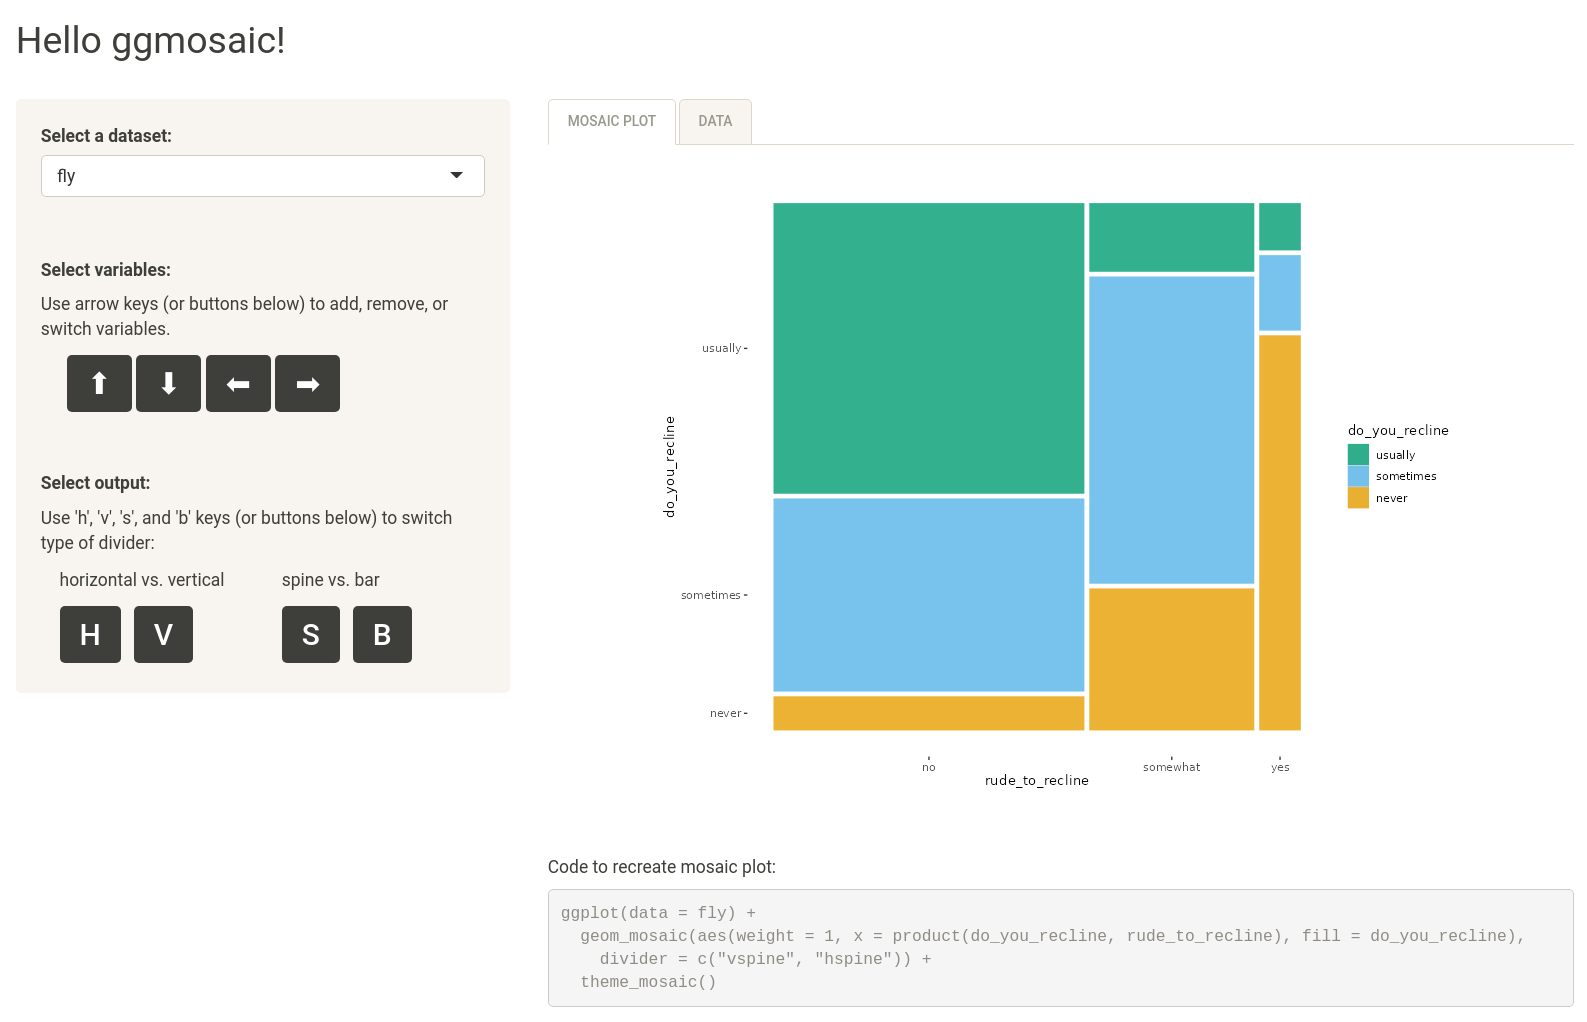
\includegraphics[width=1\linewidth]{app} 

}

\caption{A snapshot of the Shiny application that can be launched with the function \code{ggmosaic\_app()}. The Shiny app facilitates learning how to create mosaic plots. The user can explore one of three data sets provided with the package with mosaic plots created and modified via keystrokes or buttons, and no coding is required.}\label{fig:app}
\end{figure}

The app is organized into two tabs (Figure \ref{fig:app}), ``MOSAIC PLOT'' and ``DATA'', setting the stage for data set and variable selection. Creating a mosaic plot consists of several steps. Using the drop-down menu provided on the left-hand side, the user first selects from one of the three data sets exported with \pkg{ggmosaic}, the \texttt{titanic} data set, the \texttt{happy} data set, or the \texttt{fly} data set (the default selection). After the data set is selected, the user can create mosaic plots by selecting various variables to include and different dividers to be used, all completed with keystrokes or a set of buttons in the side panel.

The arrow keys (up, down, left, right) add, remove, or switch variables. The ordering of the variables can be quickly modified, allowing the user to find a sensible order for the variables in a streamlined manner. Additionally, the `h', `v', `s', and `b' keys switch the type of divider. The `h' and `v' keys switch between horizontal and vertical spines or bars, switching between `hspine' and `vpsine' or `hbar' and `vbar'. Similarly, the `s' and `b' keys can be used to select to split the categories into spines or bars, switching between `hspine' and `hbar' or `vspine' and `vbar'. If the user does not press the `h', `v', `s', or `b' keys, the `mosaic()' divider is the default, corresponding to the default divider in \texttt{geom\_mosaic()}. The `h', `v', `s', or `b' keystrokes and buttons will only affect the top-level variable. To modify the divider used on a lower-level variable, the user must backtrack via the down arrow key.

The Shiny app accommodates a better understanding of the myriad of possible forms a mosaic plot can take by accommodating a thorough search through the variables and structural changes to the mosaic plot with the simple press of certain keystrokes. The app provides an exploratory setting for visualizing many mosaic plots, and provide the user with the code necessary to recreate the selected mosaic plot.

\hypertarget{summary}{%
\section{Summary}\label{summary}}

By bringing mosaic plots into the \pkg{ggplot2} infrastructure, \pkg{ggmosaic} provides a highly customizable framework for generalized mosaic plots with a familiar syntax. The latest release of \pkg{ggmosaic} introduces novel uses of mosaic plots and exemplifies the opportunity the methods of visualizing multidimensional categorical data have for growth.

This manuscript is based on version 0.3.3 of the \pkg{ggmosaic} package. It can be installed from CRAN. The development version is available from the \href{https://github.com/haleyjeppson/ggmosaic}{GitHub repository}.

\newpage

\hypertarget{references}{%
\section{References}\label{references}}

\hypertarget{references-1}{%
\section*{References}\label{references-1}}
\addcontentsline{toc}{section}{References}

\hypertarget{refs}{}
\begin{CSLReferences}{1}{0}
\leavevmode\vadjust pre{\hypertarget{ref-ancker}{}}%
Ancker, Jessica S., Yalini Senathirajah, Rita Kukafka, and Justin B. Starren. 2006. {``Design Features of Graphs in Health Risk Communication: A Systematic Review.''} \emph{Journal of the American Medical Informatics Association} 13 (6): 608--18. \url{https://doi.org/10.1197/jamia.M2115}.

\leavevmode\vadjust pre{\hypertarget{ref-shiny}{}}%
Chang, Winston, Joe Cheng, JJ Allaire, Carson Sievert, Barret Schloerke, Yihui Xie, Jeff Allen, Jonathan McPherson, Alan Dipert, and Barbara Borges. 2021. \emph{Shiny: Web Application Framework for r}. \url{https://CRAN.R-project.org/package=shiny}.

\leavevmode\vadjust pre{\hypertarget{ref-cleveland}{}}%
Cleveland, W. S., and R. McGill. 1984. {``Graphical Perception: Theory, Experimentation and Application to the Development of Graphical Methods.''} \emph{Journal of the American Statistical Association} 79 (387): 531--54. \url{https://doi.org/10.1080/01621459.1984.10478080}.

\leavevmode\vadjust pre{\hypertarget{ref-emerson}{}}%
Emerson, John W. 1998. {``{Mosaic displays in S-PLUS: A general implementation and a case study}.''} \emph{Statistical Computing and Graphics Newsletter} 9 (1): 17--23.

\leavevmode\vadjust pre{\hypertarget{ref-friendly:history}{}}%
Friendly, Michael. 2002. {``A Brief History of the Mosaic Display.''} \emph{Journal of Computational and Graphical Statistics} 11 (1): 89--107. \url{https://doi.org/10.1198/106186002317375631}.

\leavevmode\vadjust pre{\hypertarget{ref-vcdExtra}{}}%
---------. 2016. {``{Working with categorical data with R and the vcd and vcdExtra packages}.''} In. \url{https://cran.r-project.org/web/packages/vcdExtra/vignettes/vcd-tutorial.pdf}.

\leavevmode\vadjust pre{\hypertarget{ref-galesic}{}}%
Galesic, Mirta, Rocio Garcia-Retamero, and Gerd Gigerenzer. 2009. {``Using Icon Arrays to Communicate Medical Risks: Overcoming Low Numeracy.''} \emph{Health Psychology} 28 (2): 210--16. \url{https://doi.org/10.1037/a0014474}.

\leavevmode\vadjust pre{\hypertarget{ref-hartigan}{}}%
Hartigan, John A., and Beat Kleiner. 1981. {``Mosaics for Contingency Tables.''} In \emph{Computer Science and Statistics: Proceedings of the 13th Symposium on the Interface}, 268--73. Fairfax Station, VA: Interface Foundation of North America, Inc. \url{https://doi.org/10.1007/978-1-4613-9464-8_37}.

\leavevmode\vadjust pre{\hypertarget{ref-hartigan84}{}}%
---------. 1984. {``A Mosaic of Television Ratings.''} \emph{The American Statistician} 38: 32--35. \url{https://doi.org/10.1080/00031305.1984.10482869}.

\leavevmode\vadjust pre{\hypertarget{ref-fivethirtyeight}{}}%
Hickey, Walt. 2014. {``41 Percent of Fliers Think You're Rude If You Recline Your Seat.''} \emph{FiveThirtyEight}. \url{http://fivethirtyeight.com/datalab/airplane-etiquette-recline-seat/}.

\leavevmode\vadjust pre{\hypertarget{ref-heike:03}{}}%
Hofmann, Heike. 2003. {``Constructing and Reading Mosaicplots.''} \emph{Computational Statistics and Data Analysis} 43 (4): 565--80. \url{https://doi.org/10.1016/S0167-9473(02)00293-1}.

\leavevmode\vadjust pre{\hypertarget{ref-hummel}{}}%
Hummel, Jürgen. 1996. {``Linked Bar Charts: Analysing Categorical Data Graphically.''} \emph{Computational Statistics} 11 (1): 23--33.

\leavevmode\vadjust pre{\hypertarget{ref-kleiner1981}{}}%
Kleiner, B., and J. A. Hartigan. 1981. {``Representing Points in Many Dimensions by Trees and Castles.''} \emph{Journal of the American Statistical Association} 76 (374): 260--69. \url{https://doi.org/10.1080/01621459.1981.10477638}.

\leavevmode\vadjust pre{\hypertarget{ref-yardstick}{}}%
Kuhn, Max, Davis Vaughan, and Emil Hvitfeldt. 2022. \emph{Yardstick: Tidy Characterizations of Model Performance}. \url{https://CRAN.R-project.org/package=yardstick}.

\leavevmode\vadjust pre{\hypertarget{ref-vcd}{}}%
Meyer, David, Achim Zeileis, and Kurt Hornik. 2020. \emph{Vcd: Visualizing Categorical Data}. \url{https://CRAN.R-project.org/package=vcd}.

\leavevmode\vadjust pre{\hypertarget{ref-eikosograms}{}}%
Oldford, Wayne, Erle Holgersen, Ben Lafreniere, and Tianlu Zhu. 2018. \emph{Eikosograms: The Picture of Probability}. \url{https://CRAN.R-project.org/package=eikosograms}.

\leavevmode\vadjust pre{\hypertarget{ref-playfair}{}}%
Playfair, William, Howard Wainer, and Ian Spence. 2005. \emph{Playfair's Commercial and Political Atlas and Statistical Breviary}. Cambridge University Press.

\leavevmode\vadjust pre{\hypertarget{ref-lattice}{}}%
Sarkar, Deepayan. 2020. \emph{Lattice: Trellis Graphics for r}. \url{https://CRAN.R-project.org/package=lattice}.

\leavevmode\vadjust pre{\hypertarget{ref-latticeExtra}{}}%
Sarkar, Deepayan, and Felix Andrews. 2016. \emph{{latticeExtra: Extra Graphical Utilities Based on Lattice}}. \url{https://CRAN.R-project.org/package=latticeExtra}.

\leavevmode\vadjust pre{\hypertarget{ref-carson}{}}%
Sievert, Carson. 2020. \emph{Interactive Web-Based Data Visualization with {R}, Plotly, and Shiny}. Chapman; Hall/CRC. \url{https://plotly-r.com}.

\leavevmode\vadjust pre{\hypertarget{ref-plotly}{}}%
Sievert, Carson, Chris Parmer, Toby Hocking, Scott Chamberlain, Karthik Ram, Marianne Corvellec, and Pedro Despouy. 2016. \emph{Plotly: Create Interactive Web Graphics via 'Plotly.js'}. \url{https://CRAN.R-project.org/package=plotly}.

\leavevmode\vadjust pre{\hypertarget{ref-ggrepel}{}}%
Slowikowski, Kamil. 2021. \emph{Ggrepel: Automatically Position Non-Overlapping Text Labels with 'Ggplot2'}. \url{https://CRAN.R-project.org/package=ggrepel}.

\leavevmode\vadjust pre{\hypertarget{ref-urbanek}{}}%
Theus, Martin, and Simon Urbanek. 2009. \emph{Interactive Graphics for Data Analysis: Principles and Examples}. Chapman \& Hall/CRC Computer Science \& Data Analysis. CRC Press.

\leavevmode\vadjust pre{\hypertarget{ref-atlas1870}{}}%
United States Census office. 9th census, 1870, and Francis Amasa Walker. 1874. {``{Statistical atlas of the United States based on the results of the ninth census, 1870 with contributions from many eminent men of science and several departments of the government}.''} digitized version provided through Library of Congress, \url{https://www.loc.gov/item/05019329/}.

\leavevmode\vadjust pre{\hypertarget{ref-wickham:grammar}{}}%
Wickham, Hadley. 2010. {``A Layered Grammar of Graphics.''} \emph{Journal of Computational and Graphical Statistics} 19: 3--28. \url{https://doi.org/10.1198/jcgs.2009.07098}.

\leavevmode\vadjust pre{\hypertarget{ref-ggplot2}{}}%
Wickham, Hadley, Winston Chang, Lionel Henry, Thomas Lin Pedersen, Kohske Takahashi, Claus Wilke, Kara Woo, Hiroaki Yutani, and Dewey Dunnington. 2020. \emph{Ggplot2: Create Elegant Data Visualisations Using the Grammar of Graphics}. \url{https://CRAN.R-project.org/package=ggplot2}.

\leavevmode\vadjust pre{\hypertarget{ref-productplots:paper}{}}%
Wickham, Hadley, and Heike Hofmann. 2011. {``Product Plots.''} \emph{IEEE Transactions on Visualization and Computer Graphics} 17 (12): 2223--30. \url{https://doi.org/10.1109/tvcg.2011.227}.

\leavevmode\vadjust pre{\hypertarget{ref-productplots}{}}%
---------. 2016. \emph{Productplots: Product Plots for r}. \url{https://CRAN.R-project.org/package=productplots}.

\leavevmode\vadjust pre{\hypertarget{ref-wilkinson:grammar}{}}%
Wilkinson, Leland. 1999. \emph{The Grammar of Graphics}. Springer New York. \url{https://doi.org/10.1007/978-1-4757-3100-2}.

\end{CSLReferences}

\bibliography{jeppson-hofmann.bib}

\address{%
Haley Jeppson\\
Department of Statistics\\%
Iowa State University\\ 2438 Osborn Dr\\ Ames, IA 50011\\
%
%
\textit{ORCiD: \href{https://orcid.org/0000-0003-2524-4063}{0000-0003-2524-4063}}\\%
\href{mailto:hjeppson@iastate.edu}{\nolinkurl{hjeppson@iastate.edu}}%
}

\address{%
Heike Hofmann\\
Department of Statistics\\%
Center for Statistics and Applications in Forensic Evidence\\ Iowa State University\\ 2438 Osborn Dr\\ Ames, IA 50011\\
%
%
\textit{ORCiD: \href{https://orcid.org/0000-0001-6216-5183}{0000-0001-6216-5183}}\\%
\href{mailto:hofmann@iastate.edu}{\nolinkurl{hofmann@iastate.edu}}%
}
